
\documentclass[10pt,conference,a4paper,onecolumn]{article}%{IEEEtran} % altura de letra=10, conferencia, formato a4. "`argencon"' o "`IEEEtran"' es la clase del monumento, que si no es el estandar, tiene sus propias opciones, como "`conference"'.journal
\usepackage[lmargin=2.5cm,rmargin=1.5cm,top=1.5cm,bottom=1.5cm]{geometry} % es para acomodar los margenes

% Para comentar un codigo rapido es con ctrl+q y para descomendar es con ctrl+w
%\newcommand{\CLASSINPUTbottomtextmargin}{10mm} % redefino el margen inferior
%\usepackage[latin1]{inputenc} %acentos sin codigo extra
%\usepackage[cp1252]{inputenc}% utf8
\usepackage[utf8]{inputenc} %acentos sin codigo extra \usepackage[utf8]{inputenc}
\usepackage[compress]{cite} %Es para agregar la bibliografia al final
\usepackage{url} % para poner URL 
%\usepackage[pdftex]{graphicx} % PDFLaTeX
%\usepackage[dvipdfmx]{graphicx} % PDFLaTeX

%\usepackage[dvips]{graphicx} % LaTeX
%\DeclareGraphicsExtensions{.eps}

\usepackage{graphicx}%es para agregar imagenes
\usepackage{subcaption}  %es para las subfiguras
%\usepackage{subfigure}  %es para las subfiguras
%\DeclareGraphicsExtensions{.eps,.png}
%\DeclareGraphicsExtensions{.png,.eps}
%\usepackage[spanish]{babel} % es para castellanizar algunos comandos
%\usepackage[spanish, es-tabla]{babel} % para que en vez de cuadro diga tabla
\usepackage[spanish,es-noshorthands,es-tabla]{babel} %agrega unos caracteres extra al spanish de babel
\usepackage{alltt} %Ver para que es esto, me parece que simplifica el "` vervatim"'
\usepackage{listings} % es para poder cargar los codigos y que se vean bonitos
%\usepackage{eps}  
\usepackage{chngcntr} % para los pies de pagina
\usepackage[hidelinks]{hyperref} % para agregar links "`[hidelinks]"' sirve para sacar el recuadro alrededor del link
\usepackage{amsthm} % ambiente matematico
\usepackage{amsmath} %otro ambiente matematico
%\usepackage{slashbox} % Es para poner la linea en la tabla
\usepackage[compress]{cite} %Es para agregar la bibliografia al final
%\usepackage{hyperref} % para poner un indice con que linkee a todo el texto en el pdf
\usepackage{color} % para poner textos con color 
\usepackage{hyperref} % para poner links
\usepackage{epsfig} % para poner color en las tablas
\usepackage{multirow}% para poner color en las tablas
\usepackage{colortbl}% para poner color en las tablas. Esta es la mas importante 
%\columncolor[Modelo]{Color}[SepIzq][SepDer] (columnas) \rowcolor[Modelo]{Color}[SepIzq][SepDer] (filas) 
% http://metodos.fam.cie.uva.es/~latex/apuntes/apuntes10.pdf
\usepackage[table]{xcolor}% para poner color en las tablas % http://ctan.org/pkg/xcolor
% ------------------- \newcommand
%\renewcommand{\tablename}{Tabla} % para que diga tabla en vez de ``cuadro''
\newcommand{\be}{\begin{equation}}  %Simplifica la escritura de ecuaciones
\newcommand{\ee}{\end{equation}}  %Simplifica la escritura de ecuaciones
\newcommand{\nbe}{\begin{equation*}}  %Simplifica la escritura de ecuaciones
\newcommand{\nee}{\end{equation*}}  %Simplifica la escritura de ecuaciones
\newcommand{\m}{\begin{bmatrix}}
\newcommand{\fm}{\end{bmatrix}}
\newcommand{\fig}[4]{ % Figuras asi se usa: \fig{Nombrefigura}{epigrafe}{donde? h, t, b, htb}{ancho}
\begin{figure}[#3]
\centering
\includegraphics[width=#4\columnwidth]{./Figuras/#1}
\caption{#2}\label{fig:#1}
\end{figure}}

\newcommand{\arr}[2]{ % es para poder apilar ecuaciones NO numeradas
\begin{equation*}
\begin{array}{#1} #2 
\end{array}
\end{equation*}}

\newcommand{\pap}{paso a paso\  }
\newcommand{\Mic}{microstepping}
\newcommand{\xx}{\cellcolor{blue!50}}

% --------------- FIN \newcommand ----------------------




\begin{document} % comienza el documento, es como el main.

%\title{Informe del Trabajo/Proyecto Final \\
%Accionamiento eléctrico para un motor paso a paso unipolar de reluctancia
%variable} % (?)


%\vspace{1cm} % Doy un espacio de 1cm de altura entre el titulo y el autor
\begin{titlepage}
\centering
\begin{Huge}
 
\textbf{Informe de Trabajo Final}  \\

\end{Huge}


\vspace{2cm}
\begin{figure}[h]
\centering

\includegraphics[width=3cm]{./imagenes/LogoUNC}
\end{figure}

\vspace{2cm}
\normalsize
\begin{LARGE}


 Sistemas controlados por computadora \\


 
 \end{LARGE}
 \vspace{2cm}
\begin{Large}
Diseño e implementación de un robot seguidor de linea controlado mediante PID
\end{Large}
\vspace{2cm}
\normalsize 
\begin{flushleft}
Alumnos: Tania Ferreira,  Sansoni Sebastián 

\end{flushleft}

\vspace{1cm}


\centering Neuquén, \the\year \\


\vspace{1cm}



\end{titlepage}
  % \mbox es para que no corte la oracion 
%\author{Sansoni Sebastián \\
%\emph{Maquinas Eléctricas, Ingeniería Electrónica}\\ \emph{Docentes a cargo:  Ing. Labriola Carlos, Ing. Ávila Marcelo}\\ \emph{Año 2017} \\
%\emph{ Departamento de Electrotecnia, Facultad de ingeniería, Universidad Nacional del Comahue }\\ \emph{Buenos Aires 1400, Neuquén Capital, Argentina}\\ \emph{\small{\texttt{sansoni.sebas@gmail.com}}}} 

%\author{\IEEEauthorblockN{Sansoni Sebastián} %\vspace{0.2cm}
%\IEEEauthorblockA{\emph{Maquinas Eléctricas, Ingeniería Electrónica}\\ \emph{Docentes a cargo:  Ing. Labriola Carlos, Ing. Ávila Marcelo}\\ \emph{Año 2017} \\
%\emph{ Departamento de Electrotecnia, Facultad de ingeniería, Universidad Nacional del Comahue }\\ \emph{Buenos Aires 1400, Neuquén Capital, Argentina}\\ \emph{\small{\texttt{sansoni.sebas@gmail.com}}}}} 

% en este entorno, ademas del nombre del autor se agregan mas caracteristicas en el titulo, por eso estan los "`bloques del autor"'. "`\IEEEauthorblockN"' pone los nombres. "`\IEEEauthorblockA{}"' las Afiliaciones (todo lo demas).\\ agrega un enter
%\maketitle % Dice donde poner el \emph{titulo}

%\newpage % comenzar una nueva pagina 

%\tableofcontents

%\newpage

%\begin{abstract}

%\end{abstract}
%\begin{IEEEkeywords}Actitud, acelerómetro, estimación, seguimiento\end{IEEEkeywords}




%\section{Ideas}
%Cuestiones Importantes:
%\begin{itemize}
%
%
%
%\item	Modelado del sistema (cinemático vs dinámico). Robot no holonómico.
%\item	Modelado de los motores. Ensayos con carga y sin carga.
%\item	Sistema de medición de RPM y línea.
%\item	Problema del delay en la medición de los encoders.
%\item	Ziegler-Nichols: para los motores no andaba bien por el delay variable, para el sistema total no lo podíamos implementar.
%\item	PID tuner: una vez estimado el sistema da buenos resultados.
%\item	Discretización del PID: el Tf era FUNDAMENTAL para el sistema completo.
%\item	Identificación del sistema completo.
%\item	Hipótesis simplificativas.
%\item	Controlador final.
%\end{itemize}

\section{Resumen}
El presente informe trata el diseño y desarrollo de un robot seguidor de línea. Este trabajo se encuentra enmarcado como proyecto de final de materia de Sistemas Controlados por Computadora, materia de la carrera Ingeniería Electrónica de la Universidad Nacional del Comahue.

El objetivo de estudio para la materia era la discretización e implementación en la vida real de un controlador PID. Con esto en mente se propuso la realización de un robot seguidor de línea del estilo utilizado en diversas competencias de robótica, donde el objetivo de diseño es que el robot sea capaz de seguir una pista en un plano horizontal de forma autónoma en el menor tiempo posible. El presente trabajo se orientó a la obtención de un seguidor de línea básico, de velocidad moderada, con perspectiva de mejorarse en versiones posteriores.

\section{Introducción}
%Esto fue copiado de la propuesta presentada 19/12/17

\subsection{Motivación}
En el marco de las Jornadas Argentinas de Robótica (JAR) 2019 a realizarse en la Universidad Nacional del Comahue, se desea dar los primeros pasos en la implementación de sistemas robóticos. En particular, se desea trabajar en el inicio de un movimiento en la facultad para la utilización de la robótica educativa. \\
La robótica educativa, también conocida como robótica pedagógica, es una disciplina que tiene por objeto la concepción, creación y puesta en funcionamiento de prototipos robóticos y programas especializados con fines pedagógicos (Ruiz-Velasco, 2007). Partiéndose de un proyecto concreto a realizar, el proceso de concepción, diseño, armado y puesta en marcha del prototipo enriquece el proceso de aprendizaje del alumno, fortaleciendo sus capacidades de liderazgo y motivándolo a resolver retos cada vez más
complejos. \\
Este tipo de herramienta pedagógica se encuentra dentro de la metodología ABP (aprendizajes basados en proyectos). El ABP se desarrolla en un entorno real y experimental, lo que ayuda a los alumnos a relacionar los contenidos teóricos con el mundo real y mejora la receptividad para aprender los conceptos teóricos. Los alumnos toman un papel activo en el proyecto, ya que tienen que marcar el ritmo y profundidad del aprendizaje, y fijar los objetivos de la realización del proyecto. Este tipo de metodología motiva al alumno, por lo que resulta una estrategia de particular interés para mejorar el rendimiento académico y la persistencia
en los estudios. \\
En la UNCo, particularmente en nuestra carrera, existe una fuerte inclinación a priorizar la enseñanza de conceptos casi exclusivamente teóricos, habiendo actualmente pocas materias que pidan la realización de proyectos concretos. Este enfoque puede traer aparejado una serie de inconvenientes: alumnos con poca capacidad para resolución de problemas reales, dificultad para relacionar los conceptos aprendidos con la vida real o para entender los mismos, falta de motivación en los alumnos, etc. Considerando esto y que actualmente la tasa de deserción en la carrera es de 50 o más\%, es que se desea avanzar hacia las metodologías
ABP mencionadas, particularmente en el área de robótica. \\
En el marco de esto, el presente trabajo busca implementar los conocimientos adquiridos en la materia en el diseño e implementación de distintas estrategias de control sobre un robot en la configuración de seguidor de línea.
 \subsection{Seguidor de línea}
 Los robots seguidores de línea son robots muy sencillos, que cumplen una única misión: seguir una línea marcada en el suelo (normalmente de color negro sobre un tablero blanco). Son considerados los "Hola mundo" de la robótica. La dificultad del recorrido determina la complejidad del robot y el requerimiento o no de una mayor cantidad de sensores, capacidad de procesamiento, mejoras de hardware, etc. Esta flexibilidad los hace particularmente interesantes como herramientas educativas, ya que se puede comenzar con diseños sencillos para luego avanzar en sucesivas mejoras del prototipo, pudiendo adaptarse a distintas materias de
la carrera.\\
En Argentina se festejan distintas competencias relacionadas con la fabricación y puesta en marcha de los seguidores de líneas, también clasificada como la modalidad “carreras”. Se destacan entre otros:
\begin{itemize}
\item $15^o$ Competencia Internacional de Robótica - GRS - UTN Bahía Blanca.
\item Liga nacional de robótica - \url{http://www.lnr-argentina.com.ar}
\item Competencia Nacional de Robótica 2017 - Instituto La Salle Florida – Bs. As.
\item Grupo de Robotica Universidad de Mendoza (GRUM).
\item Instituto Tecnológico del Comahue (ITC)- Neuquen.
\end{itemize}
A nivel internacional existe un proyecto llamado Open Lamborghuino \cite{lambo}, en el cual se detalla la construcción
de un seguidor de línea con componentes relativamente baratos y de fácil acceso.

\section{Objetivos de la propuesta}
\label{objetivos}
\begin{itemize}
\item Desarrollar e implementar un robot seguidor de linea.
\item Identificación y modelado del sistema.
\item Implementar un controlador PID discreto.

\end{itemize}
\section{Estructura del Trabajo}
El siguiente trabajo se divide en {\color{red}XXXX secciones}. En la sección \ref{sec:implementacion} se define el hardware y estructura mecánica a utilizar, con un detalle del material de trabajo disponible. En la sección \ref{sec:Modelado_del_sistema} se analiza cómo modelar matemáticamente el comportamiento del sistema. En  \ref{sec:estrategia_de_control} se define la estrategia de control a implementar. En \ref{sec:sist_de_medicion} se explican los sensores diseñados para el robot. En \ref{sec:identifSist} se aborda la identificación de sistemas realizada para poder ajustar los controladores, lo cual se detalla en la sección \ref{sec:ajus_control}. Finalmente, la sección \ref{sec:resultados} discute los resultados obtenidos al probar el sistema completo, mientras que en la sección \ref{sec:conclusiones} se dan las conclusiones del trabajo.

\section{Implementación}
\label{sec:implementacion}
Para facilitar la implementación del robot, se propone utilizar la configuración de hardware recomendada en open lamborghino con algunas modificaciones de diseño propio. La configuración se detalla a continuación:
\begin{itemize}
\item 2 motores N20 con reducción 1:10 \cite{motores}. 
\item Driver para motores: TB6612FNG \cite{puenteH}.
\item Computadora de abordo: Arduino Nano \cite{arduinoNano}.
\item Batería de LiPo: 2S 1100mA.
\item Comunicación inalámbrica: par de Módulos bluetooth HC-05 o similar.  
\item Estructura fabricada en la impresora 3D de la facultad.

\end{itemize}

\subsection{Estructura Mecánica}%$.$ Mejorar el nombre
Se definió utilizar una estructura con dos ruedas y un punto de apoyo. El frente del robot se encuentra en el lado opuesto al del punto de apoyo, con una estructura para soporte de los LEDs del sensor de línea colocada en esta zona. La estructura diseñada se muestra en la figura \ref{fig:estructuraRobot}.
\begin{figure}[h] %$.$ Faltan los encoders
\centering
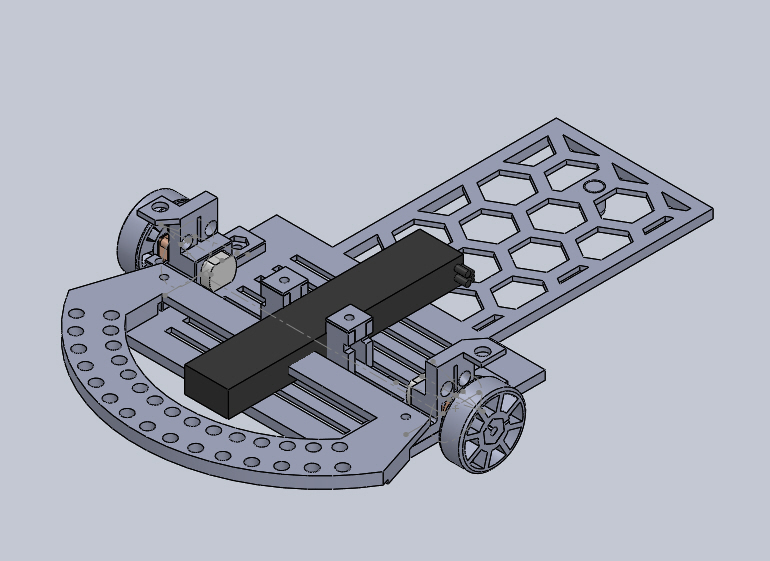
\includegraphics[width=8cm]{./imagenes/estructuraCompleta.png}
\caption{Estructura mecánica del robot.}
\label{fig:estructuraRobot}
\end{figure}
El diseño de las piezas mecánicas fue realizado por el ahora ingeniero Carrascal Cliver. Las mismas se imprimieron con impresora 3D.
\section{Modelado del sistema} \label{sec:Modelado_del_sistema}
%Las ecuaciones cinemáticas son aquellas que relacionan la velocidad de giro de cada una de las ruedas con las variables de posición del robot en el plano.
%\begin{equation}
%\vec{x}= (x,y,\phi )
%\end{equation}
 
%Considerando al robot como un cuerpo rígido, la velocidad lineal del centro de masa se obtiene a partir del promedio de las velocidades lineales de cada una de sus
%ruedas. La velocidad lineal de cada rueda se obtiene como el producto de la velocidad angular (velocidad de giro) y el radio de ellas. La velocidad del centro de masa
%queda definida por:
%\begin{equation}
%V_{cm}= \frac{r}{2} (w_l-w_r) 
%\end{equation}

\subsection{Modelo cinemático}
\label{modelo cinematico}
\subsubsection{Ecuaciones de Movimiento}
% Agregado, es un choreo de pathfoll
Según \cite{pathfoll}, el robot que se desea modelar se lo conoce como robot diferencial ya que cuenta con 2 ruedas y un punto de apoyo. Esta clase de robots son no holonómicos ya que tiene restricciones a la hora de realizar movimientos sobre el plano; por ejemplo, no puede realizar movimientos puramente laterales. En la figura \ref{fig:robot_diferencial} se muestra un esquemático de este tipo de robots.
\begin{figure}[h]
\centering
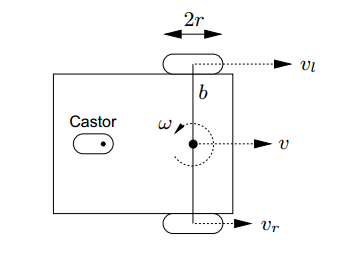
\includegraphics[width=6cm]{./imagenes/robot_diferencial.png}
\caption{Robot diferencial. }%\cite{pathfoll} .}
\label{fig:robot_diferencial}
\end{figure}

Suponiendo que no hay deslizamiento, la posición y orientación del punto central del dispositivo, C, están dadas por las ecuaciones cinemáticas \ref{eq:ec_cinem}. El punto C es el punto medio del segmento que une las ruedas del robot.

\begin{equation}
\dot{x}=v\cos\theta \quad \dot{y}=v\sin\theta \quad \dot{\theta}=\omega
\label{eq:ec_cinem}
\end{equation}

Donde $(x,y)$ indica la posición del centro C en el espacio carteciano y $\theta $, conocida como orientación, es el angulo entre el eje $x$ del sistema de cordenadas y el eje homologo del robot, es decir, el eje de simetría del cuerpo.  De esta manera $(x,y,\theta)^T$ definen la postura del sistema completo.

 Si los motores se mueven a velocidades $\omega_R$ y $\omega_L$, las velocidades $v$ y $\omega$ son \cite{planning}:

\begin{equation*}
v=\frac{r(\omega _R + \omega _L)}{2}
\end{equation*}


\begin{equation}
\label{wc}
\omega_{C}=\frac{r(\omega _R - \omega _L) }{L}
\end{equation}

donde L es la distancia entre las ruedas. 

\subsubsection{Modelado del sistema de medición }%$.$ Mejorar nombre
\label{sec:modelo_orien}
Suponiendo la situación mostrada en la figura \ref{fig:posturas} en donde la linea a seguir se encuentra sobre el eje $x$, 

\begin{figure}[h]
\centering
    \begin{subfigure}[h]{0.45\textwidth}
    	\centering
        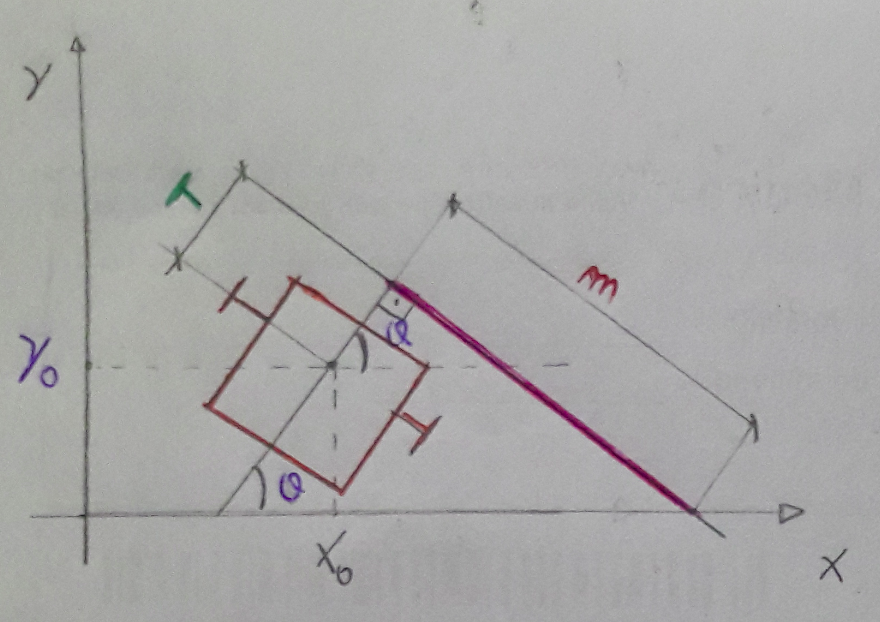
\includegraphics[width=7.5cm]{./imagenes/geometria_A.png}
        \caption{}
    \end{subfigure}
    \quad
    \begin{subfigure}[h]{0.45\textwidth}
    	\centering
        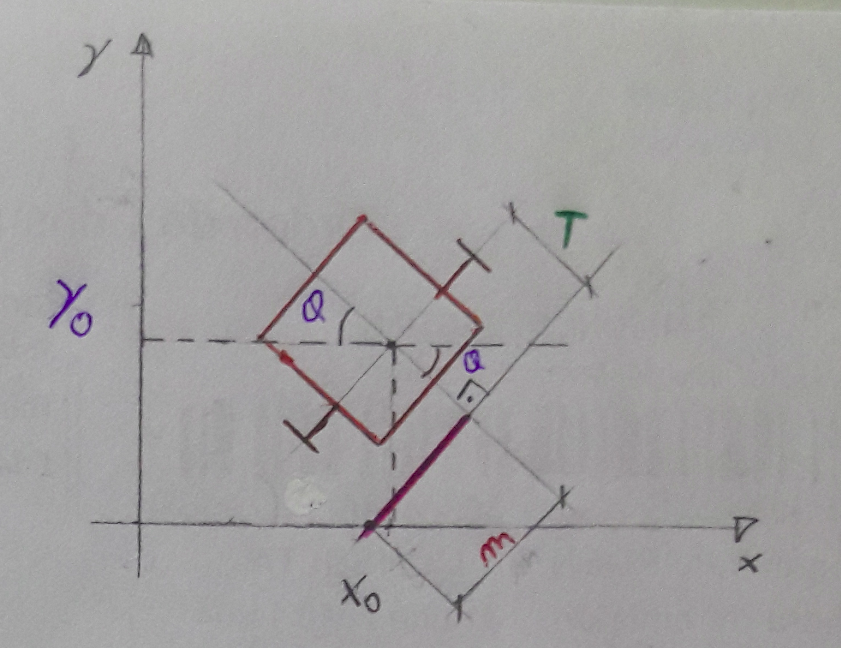
\includegraphics[width=7.5cm]{./imagenes/geometria_B.png}
        \caption{}
    \end{subfigure}
    \caption{Geometría del robot considerando dos posturas distintas: (a) $Y_0 >0 $ y $ \theta >0 $ y (b) $Y_0 >0$ y $ \theta <0$.}
	\label{fig:posturas}
\end{figure}

con ayuda de un poco de geometría se puede demostrar que para (a) 

\begin{equation}
m= \left( T\sin(\theta) + Y_0 \right) \frac{1}{\cos(\theta)}
\label{eq:pose1}
\end{equation}

y para (b)

\begin{equation}
m=\sqrt{Y_0^2 - T^2 + \left((T-Y_0\sin(\theta))\frac{1}{\cos(\theta)} \right)^2}
\label{eq:pose2}
\end{equation}

en donde $m$ es la medida del sensor en \textit{metros}, $\theta$, $X_0$ y $Y_0$ determinan la pose del dispositivo. 

Suponiendo que $ | Y_0 | \approx 0$ y simplificando en \ref{eq:pose1} y \ref{eq:pose2}  resulta que

\begin{equation}
m \approx T \tan(\theta)
\end{equation} 

%Dado que el único sensor disponible es el sensor de línea, no se tiene la información completa para trabajar con las ecuaciones \ref{eq:ec_cinem}. En función de esto se decidió plantear una hipótesis simplificativa que permitiese estimar la orientación del vehículo respecto a la pista. Se decidió trabajar con esta variable porque la ecuación que gobierna la orientación del robot es LTI y si la pista es una línea recta la orientación relativa a esta respondería a la misma ecuación.

%Las hipótesis a utilizar son que la pista es una línea recta y que el centro C del vehículo se encuentra siempre sobre el centro de la linea a seguir. Así, la señal de error $e$ se toma como la distancia entre el eje central del robot y el punto de intersección entre la línea de sensores y la recta a seguir. Esta situación se muestra en la figura \ref{fig:carrito1}.

%\begin{figure}[h]
%\centering
%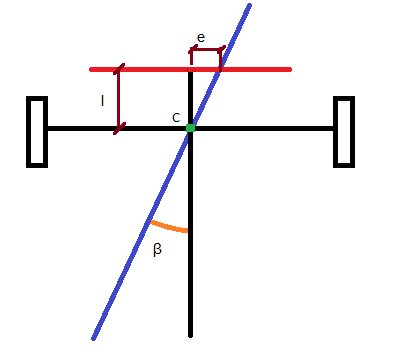
\includegraphics[width=10cm]{./imagenes/carrito1.png}
%\caption{Esquema del robot sobre la línea a seguir (azul). La línea roja representa la línea de sensores, $e$ es la distancia medida entre el eje central del robot y la intersección de la recta a seguir con la línea de los sensores, y $\beta $ es el ángulo entre la línea a seguir y el eje central del robot.}
%\label{fig:carrito1}
%\end{figure}
%
%Bajo la hipótesis de que la pista es una línea recta, la relación entre $\beta$ y la orientación del robot $\theta$ está dada por: \begin{equation*}
%\beta=\theta-\psi
%\end{equation*}
%Donde $\psi$ es la orientación de la pista. Como $\psi$ es constante, reemplazando en \ref{eq:ec_cinem} obtendríamos:
%
%\begin{equation}
%\label{betaDerivada}
%\dot{\beta}=\omega_C
%\end{equation}
%
%Dado que sólo se tiene la medición de $e$, se utiliza la segunda hipótesis propuesta: que el punto C se mantiene siempre sobre la línea a seguir. Bajo esta suposición, podemos calcular $\beta $ por trigonometría:
%
%\begin{equation*}
%\tan(\beta)=\frac{e}{l}
%\end{equation*}

Como $T$ es fijo, la medición de $m$ puede traducirse en una medición del ángulo de orientación. De esta manera podríamos buscar minimizar el ángulo para alinear el robot con la pista. Como la medición se hace suponiendo que $Y_0 \approx 0 $, si el robot no está centrado respecto a la pista el cálculo del ángulo va a indicar una medición errónea, por lo que al llevar a cero $ \theta $ medido de esta manera se termina garantizando que el robot esté centrado respecto a la pista.

La hipótesis utilizada debería ser válida si el sistema controlado es lo suficientemente rápido para corregir desviaciones antes de que el centro se desplace fuera de la pista.

Como lo que se controla son las velocidades de cada motor de forma individual, resulta que


\begin{equation}
\dot{\theta}=\omega_C=\frac{r(\omega _R - \omega _L)}{L}
\label{eq:tita_omega}
\end{equation}

dado que solo  interesa la diferencia entre velocidades angulares del motor, se puede mantener $v$ constante (por medio de $\omega $) tomando:

\begin{equation*}
\omega _R = \omega _{fijo} + \frac{\Delta \omega}{2} 
\end{equation*}

\begin{equation*}
\omega _L = \omega _{fijo} -\frac{\Delta \omega}{2}
\end{equation*}

Esto disminuiría el problema a una sola señal de control $\Delta \omega$.

\subsubsection{Radio de giro}
En la figura \ref{fig:girando} se muestra la disposición del robot cuando esta siguiendo una curva.
\begin{figure}[h]
\centering
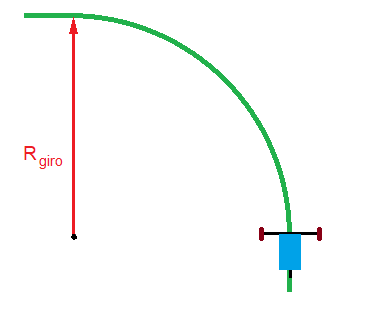
\includegraphics[width=7cm]{./imagenes/carrito_girando.png}
\caption{Esquema del robot girando.}
\label{fig:girando}
\end{figure}
En este caso la velocidad del punto C tiene una componente tangencial, $v$, y una componente radial, $\omega$, dadas por

\begin{equation}
v =\frac{r(\omega _R + \omega _L) }{2}=r \omega_{fijo}
\label{eq:v_tan}
\end{equation}

\begin{equation}
\omega_{C} =\frac{r(\omega _R - \omega _L) }{L}= \frac{  r \Delta \omega} {L}
\label{eq:omegac}
\end{equation}

 la relación entre ambas magnitudes es


\begin{equation*}
v=R_{giro} \omega_{C}
\end{equation*}

reemplazando esto en las ecuaciones \ref{eq:v_tan}  y \ref{eq:omegac}, se obtiene
\begin{equation}
\Delta \omega= \frac{\omega_{fijo}L}{R_{giro}}
\end{equation}

Así, mientras más pequeño sea el radio de giro, más grande debe ser $\Delta \omega$. Para una velocidad $\omega_{fijo}$ constante, el máximo valor admisible de $\Delta \omega$ determinará el menor radio de giro que podrá hacer el robot.

 \subsection{Modelado de los motores}
 \label{modeloMotores}
 
 Los motores a utilizar son motores de DC con escobillas. Según \cite[pág. 58-59]{dorf}, si se desprecia el torque de la perturbación,%$.$ para mí no se entiende qué es el torque de "perturbación", pero no sé qué es exactamente como para poder cambiarlo :( (dorf pág 58-59)
\ la función de transferencia de la combinación motor-carga resulta
 \begin{equation*}
 \frac{\theta(s)}{V_f(s)}=\frac{K_m}{s(Js+b)(L_fs+R_f)}
 \end{equation*}
 donde $\theta$ es la posición angular, $V_f$ es la tension de exitación, $K_m$ es la constante que relaciona la corriente con el par del motor, $J$ es el momento de inercia del eje, $b$ es la constante de fricción del eje, $L_f$  y $R_f$ son la autoinductancia y resistencia del bobinado, respectivamente. Simplificando la función de transferencia resulta
 \begin{equation*}
 \frac{\theta(s)}{V_f(s)}=\frac{k}{s(s+a)(s+b)}
 \end{equation*}
 donde $k$, $a$ y $b$ son constantes a determinar mediante la identificación.
 
Por practicidad en vez de usar $\theta$ se usa $\dot{\theta}$, lo que produce la siguiente función de transferencia
 \begin{equation}
 \frac{\dot{\theta}(s)}{V_f(s)}=\frac{k}{(s+a)(s+b)}
 \end{equation}
  
\section{Estrategia de Control a Utilizar}
\label{sec:estrategia_de_control}
Para alcanzar los objetivos del proyecto se decidió implementar tres controladores PID en simultáneo: dos controladores para regularizar el comportamiento de los motores y el controlador para el sistema total, que se encargará de que el robot siga la pista. Los dos primeros se utilizan para que las ruedas se muevan a la velocidad requerida y para compensar asimetrías en la respuesta de los dos motores.
Una vez implementados todos los controladores descritos el sistema total queda según se observa en el diagrama en bloque de la figura \ref{diagra en bloques sist total}.
\begin{figure}[h]
\centering
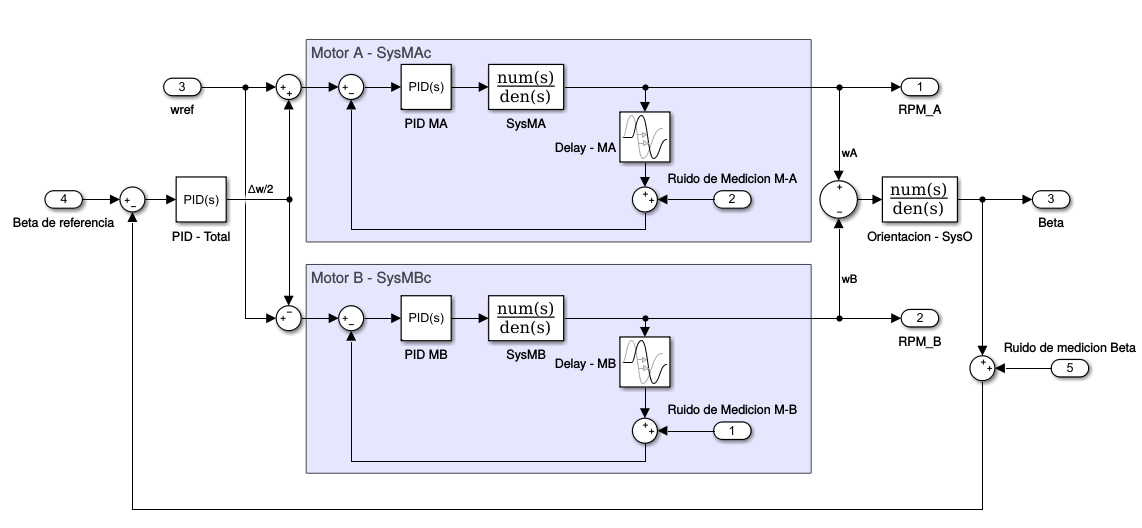
\includegraphics[height=7cm]{./imagenes/sistema_total}
\caption{Diagrama en bloques del sistema total con los tres controladores PID implementados.}
\label{diagra en bloques sist total}
\end{figure}

En la anterior figura, se observa que cada sistema motor $Sys_M$ cuenta con dos entradas, una llamada $\omega_{ref}$ y otra $\pm \frac{\Delta \omega}{2}$, ademas cuentan con su propia controlador, originando así un sistema realimentado llamado $Sys_{Mc}$. Luego la diferencia de velocidades de los  ejes de cada motor controlado ingresa a la planta de orientación $Sys_O$. Con ayuda de la ecuación \ref{eq:tita_omega}  se deduce:

\begin{equation}
\theta=Sys_O(\omega_R - \omega_L)=Sys_O\left( Setpoint_BSys_{MBc} - Setpoint_ASys_{MAc}   \right)
\end{equation}

en donde $Setpoint = \omega_{ref} \pm \frac{\Delta \omega}{2}$, luego reemplazando


\begin{equation}
\theta=Sys_O\left(Sys_{MBc}(\omega_{ref}+\frac{\Delta \omega}{2}) - Sys_{MAc} (\omega_{ref}-\frac{\Delta \omega}{2}) \right)
\end{equation}

reordenando

\begin{equation}
\theta=Sys_O\left(\omega_{ref} (Sys_{MBc}-Sys_{MAc})+  \frac{\Delta \omega}{2}( Sys_{MBc}+Sys_{MAc})  \right)
\end{equation}

luego si $Sys_{MBc} \approx Sys_{MAc}$ y ademas el termino $\omega_{ref} (Sys_{MBc}-Sys_{MAc})$ es muy pequeño comparado con $ \frac{\Delta \omega}{2}( Sys_{MBc}+Sys_{MAc}) $ resulta que

\begin{equation}
\theta=\Delta \omega Sys_OSys_{MAc}= \Delta \omega Sys_{total}
\end{equation}

por lo tanto es necesario que el sistema controlado de ambos motores se comporten lo mas parecido posible y que ademas se cumpla $\omega_{ref} (Sys_{MBc}-Sys_{MAc}) \ll  \frac{\Delta \omega}{2}( Sys_{MBc}+Sys_{MAc}) $.

Bajo estas hipótesis, el sistema completo sin control en la orientación será

\begin{equation}
\frac{\theta(s)}{\Delta \omega (s)}=Sys_O(s)Sys_{MAc}(s)=Sys_O(s)\frac{C_a(s)Sys_{MA}(s)}{1+C_a(s)Sys_{MA}(s)}
\label{eq:sys_tot_LA}
\end{equation}

%y con control en la orientacion 
%
%\begin{equation}
%\frac{\theta(s)}{\Delta \omega}=\frac{C_OSys_O(s)\frac{C_a(s)Sys_{MA}(s)}{1+C_a(s)Sys_{MA}(s)}}{1+C_OSys_O(s)\frac{C_a(s)Sys_{MA}(s)}{1+C_a(s)Sys_{MA}(s)}}
%\end{equation}

en donde $C_a(s)$ es el controlador para el motor $A$.
\subsection{PID}
 %Esta parte es un choreo MODIFICADO de \cite[pág. 25]{biblia_PID}.\\

En esta sección no se espera realizar un analisis profundo sobre el controlador PID, sino mas bien una intro cualitativa, con algunas referencias hacia \cite{biblia_PID}. Por otro lado se parte de la suposicion de que se conocen algunos principios fundamentales de control. %(realimentacion, lugar de las raices, polos, ceros, entre otros.)

Un controlador PID esta constituido por 3 controles facilmente identificables: Proporcional (P), Integral (I) y Derivativo (D). Si bien el nombre \textit{PID} hace referencia a la estrategia de control, existen distintas maneras de implementarlo, esto es I-PD, PI-D, PI, PD, P, entre otros. 

Por cuestiones didacticas, se explicara sinteticamente lo mas relevante de algunos de estos controladores.% (sos un choto, al final no vas a explicr nada).


Considerando la figura \ref{fig:sis_generico}, se puede observar el diagrama en bloques de un sistema generico realimentado, en donde \textit{l} y \textit{n} son ruido/perturbaciones del modelo y de la medición respectivamente,   \textit{r} es la señal de referencia, esto es, el valor deseado de la señal de salida \textit{y}; \textit{e} es la diferencia entre el valor deseado y el valor medido de la salida,    \textit{u} es la salida del controlador (o accion de control) y  \textit{x} es la salida de la planta sin que este afectada por ruidos / perturbaciones.

\begin{figure}[h]
\centering
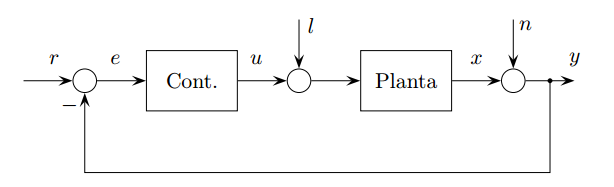
\includegraphics[height=3cm]{./imagenes/sis_realim_generico.png}
\caption{Diagrama en bloques de un sistema realimentado.}
\label{fig:sis_generico}
\end{figure}


\subsubsection{Control Proporcional}
Un control proporcional es aquel en donde la accion de control \textit{u} es proporcional al error \textit{e}, esto es

\begin{equation}
e=r-y \quad \rightarrow u=k(e)=k (r-y)
\end{equation}

Para lograr un mejor entendimiento, vamos a hacer uso de un ejemplo:
\paragraph{Ejemplo:} Se desea controlar la velocidad del eje de un motor de corriente continua (CC), para esto se cuenta con un generador de \textit{PWM} y un sistema de medicion de las \textit{RPM} del eje.

Supongamos que deseamos que el eje del motor gire a $1000RPM$, inicialmente el eje se encuentra en reposo, por lo que la medicion del sensor sera $y=0RPM$. Dados estos datos el error sera

 \begin{equation*}
e=r-y \quad \rightarrow e=1000RPM - 0RPM =1000RPM
\end{equation*}
por lo que la accion de control sera $u=k 1000RPM$.

En este caso el valor de $k$ representa una constante que adecua las unidades de \textit{RPM} a \textit{\% de duty} y ademas aplica un factor de ganancia, esto es:
 \begin{equation*}
k=k_{unidades}k_{ganancia}
\end{equation*}
 
 Dicho esto, supongamos que $k_{unidades}=1/10 \quad [\%duty/RPM]$ y que $k_{ganancia}=1$, luego la salida del controlador sera $100 \%duty$.
 
 Si todo esta bien conectado, el eje se comenzara a mover, por lo que el sensor de velocidad medirá una velocidad no nula, lo cual producira una señal de control menor a la que inicialmente se obtuvo. Luego de un periodo prudente en donde el estado transitorio convergio, se observa que la velocidad final del motor resulta ser $y=700RPM$ y la acción de control por lo tanto sera $u=k(r-y)=30\quad [\%duty]$. \\
 
 
 Gracias al anterior ejemplo se pueden observar algunas características del control proporcional:
 \begin{enumerate}
 \item \label{item_prop} Cuando el error \textit{e} es cero la salida es cero, por lo que siempre habrá una diferencia entre el valor deseado (set point) y el valor medido, a menos claro que el $set point$ sea cero.
 \item Si el valor de $k_{ganancia}$ es mas grande, en el estado estacionario se puede observar que la salida del control sera mayor, por lo que el motor girara a mayor velocidad, produciendo asi, un valor mas cercano al deseado.
 \item Si $k_{ganancia}$ es un valor elevado, cuando exista alguna perturbación en la medición, este error en la medida sera \textit{k} veces amplificado en la acción de control. 
 \end{enumerate}
 
 
 \subsubsection{Control Integral}

Para resolver la problemática planteada en el item \ref{item_prop} del control proporcional, se plantea como solución la utilización de un control integral. 

El control integral se puede interpretar como que la salida de control \textit{u} es proporcional a la integral del error \textit{e}, en símbolos


\begin{equation}
u=K_i \int_{t_0}^{t_1} e \,dt 
\label{eq:control_integral}
\end{equation}


en la cual se observa que si el error entre la salida y el set point perdura en el tiempo, la acción de control se incrementara hasta que el error sea nulo.

\paragraph{Problemática:} En la realidad, la acción de control posee una cota, ya que no puede ser arbitrariamente grande. 
Suponga el ejemplo utilizado en el \textbf{Control Proporcional}, pero esta vez tiene implementado un controlador PI y ademas hay una falla en las conexiones lo que produce que el motor no funcione. El $set point$ se establece en $1000RPM$, la acción de control es de $100\%duty$, pero como el motor esta mal conectado, el eje no gira produciendo que luego de unos instantes el error siga siendo de  $1000RPM$ y el termino integral incremente a medida que siga pasando el tiempo. Cuando se corrija la falla eléctrica, el eje del motor girará a una velocidad superior a la del $set point$ el tiempo necesario hasta que el error negativo "des-integre" todo el error acumulado anteriormente.

Como solución a esta problemática se implementan técnicas de ventaneo, tal que limiten la parte integral y no permita que diverja.  



\subsubsection{Control Derivativo}
El control derivativo, o la acción derivativa, se puede interpretar como anticiparse al error en un estado posterior al actual, por medio del calculo de la tangente de la curva del error. Para obtener esta predicción, suponga la expansión en serie de Taylor


\begin{equation*}
e(t_1)=e(t_0)+\frac{de(t_0)}{dt}(t_1-t_0)+... 
\end{equation*}
\begin{equation}
 e(t_1) \approx e(t_0)+\frac{de(t_0)}{dt}(t_1-t_0)
\end{equation}

en ella se puede apreciar que aparece un termino del error actual y luego otro termino con la derivada del error ponderada por la diferencia temporal. A este controlador se lo conoce comúnmente como PD, el cual su estructura básica se muestra a continuación

\begin{equation}
u(t)=K_pe(t)+K_d\frac{de(t)}{dt}
\end{equation}

Según \cite[pág. 40]{biblia_PID} la acción derivativa puede traer dificultades si existe ruido de medición de alta frecuencia. Un ruido de medición sinusoidal
\begin{equation*}
n=a\sin(\omega t)
\end{equation*}
contribuye al término derivativo de la señal de control como
\begin{equation*}
u_n=K_d \frac{dn}{dt}=aK_d\omega\cos(\omega t)
\end{equation*}

Podemos observar que la amplitud de la señal de control puede ser arbitrariamente grande si la frecuencia $\omega$ es suficientemente alta.

Por este motivo, es común que la ganancia del término derivativo sea limitada en alta frecuencia. Esto puede lograrse implementando el término derivativo como


\begin{equation}
D'=D_{ideal}(s)D_{sat}(s) =sK_d \quad  \frac{1}{1+s\frac{K_d}{N}} =    \frac{sK_d}{1+s\frac{K_d}{N}}
\label{eq:ajuste_deriv}
\end{equation}

Esta modificación puede interpretarse como la derivada del error del sistema concatenada con un filtro pasa bajos con un polo colocado $N$ veces mas lejos. Quiere decir que para frecuencias menores a $\frac{N}{K_d}$ la derivada del error se amplificara como antes, pero cuando la frecuencia supere esta cota, el sistema saturara. Valores normales de $N$ oscilan entre 8 y 20. % (Pensar en el bode de este sistema, no se si hace falta poner una imagen)  

\subsubsection{PID total}

Dado lo visto anteriormente, si se consideran todas las acciones de control en paralelo, el sistema para tiempo continuo resulta

\begin{equation}
u(t)=K_pe(t)+K_i \int_{t_0}^{t_1} e(t) \,dt + K_d \frac{de(t)}{dt}
\end{equation}

en donde los parámetros $K_p$, $K_i$ y $K_d$ son las constantes con las que se realiza el ajuste para cada planta en particular. 

La representación anterior es la forma clásica (o no interactuante) del controlador PID escrita para tiempo continuo. En forma de función de transferencia resulta:
\begin{equation}
G(s)e(s)=\left(K_p + K_i/s + sK_d \right)e(s)
\label{eq:pid_basico}
\end{equation}
considerando el ajuste de la ecuacion \ref{eq:ajuste_deriv}, la exprecion \ref{eq:pid_basico} resulta

\begin{equation}
G(s)e(s)=\left( K_p + K_i/s + \frac{sK_d}{1+\frac{sK_d}{N} } \right)e(s)
\label{eq:pid_final}
\end{equation}



 
 \subsubsection{Discretización PID}
% 
% \begin{itemize}
% \item Formas de discretizar
% \item discretizacion estandar, problemas
% \item Discretizacion del astrom
% \end{itemize}
 
 Según \cite[pág. 214]{astrom} se pueden representar una ecuación diferencial mediante su aproximación:
 
 \paragraph{Método de Euler:} La derivada de una variable se puede aproximar por una \textbf{diferencia adelantada}
 
 \begin{equation}
 \frac{dx(t)}{dt}\approx \frac{x(t+h)-x(t)}{h}
 \end{equation}
  
  o por  una \textbf{diferencia atrasada}
  
   \begin{equation}
 \frac{dx(t)}{dt}\approx \frac{x(t)-x(t-h)}{h}
 \end{equation}
  
  por otro lado, según \cite[pág. 46 ]{biblia_PID} la integral de una variable dada por la ecuación \ref{eq:int_var} se puede aproximar mediante  distintas formas recursivas.
  
\begin{equation}
I(t)=\frac{K}{T_i}\int_0^t e(t) \,dt
\label{eq:int_var}
\end{equation}  
  
  \paragraph{Regla rectangular hacia adelante:} 
  
  \begin{equation}
  I(nh)=\frac{K}{T_i}h \sum_0^{n-1}e(nh)= \frac{K}{T_i}h \sum_0^{n-2}e(nh) + h\frac{K}{T_i} e((n-1)h)=I((n-1)h)+  h\frac{K}{T_i} e((n-1)h)
  \end{equation}
  
  \paragraph{Regla rectangular hacia atrás:} 
  \begin{equation}
  I(nh)=\frac{K}{T_i}h \sum_0^{n}e(nh)=I((n-1)h)+  h\frac{K}{T_i} e(nh)
  \end{equation}
  Esta aproximacion se diferencia de la anterior, en que utiliza la muestra actual de la señal $e(nh)$ en vez de la muestra anterior $e(h(n-1))$.
  
  \paragraph{Regla trapezoidal:} 
  
  \begin{equation}
  I(nh)=\frac{K}{T_i}h \sum_{i=1}^{n}e((i-1)h)-e(ih)=I((n-1)h)+  \frac{K}{T_i} \frac{e(nh) -e((n-1)h)}{h}
  \label{eq:aprox_trape} 
  \end{equation}
  
  Según \cite{astrom} en el contexto del control digital la aproximación \ref{eq:aprox_trape} suele denominarse \textit{aproximación de Tustin, o transformación bilineal.} Utilizando estos métodos la funcion de transferencia discreta $H(z)$ se obtiene simplemente sustituyendo el argumento $s$ de $G(s)$ por $s'$, donde
  
  \begin{equation}
  s'=\frac{z-1}{h} \quad (Metodo\ de\ Euler)
\end{equation}   
  \begin{equation}
  s'=\frac{z-1}{zh} \quad (Diferencias\ en\ retroceso)
\end{equation}   
\begin{equation}
  s'=\frac{2}{h} \frac{z-1}{z+1} \quad (Aproximacion\ de\ Tustin)
\end{equation}  

considerando la expresión \ref{eq:pid_final} y teniendo en cuenta \cite[pág. 219]{astrom} el método más común para discretizar un PID es realizar una aproximación de Euler para la parte integral y una aproximación en diferencias en retroceso para la parte derivadora, lo cual origina el siguiente controlador discreto:

\begin{equation}
  u(kh)=\left(K_p + \frac{K_ih}{z-1} + K_d\frac{z-1}{zh+\frac{K_d}{N}(z-1)}	  \right) e(kh)
\end{equation}  

el cual por medio de manipulación algebraica se puede transformar en la siguiente ecuación en diferencias

\begin{equation}
u(k+1)=Ae(k)+Be(k-1)+Ce(k-2)+Du(k-1)+Eu(k-2)
\end{equation} 
donde los parámetros $A$,$B$,$C$,$D$ y $E$ se obtienen a partir de las constantes $h$,$Kp$,$Ki$,$Kd$ y $N$. Es conveniente utilizar algún software de cálculo como apoyo para realizar estas transformaciones.
\section{Sistemas de Medición}
\label{sec:sist_de_medicion}
\subsection{Medición de velocidad de los Motores}
\subsubsection{Estructura Mecánica}
Para la medición de velocidad de los motores se utilizaron encoders ópticos. Estos consisten en un diodo LED infrarrojo enfrentado a un fotodiodo receptor en dirección vertical, con una estructura que interrumpe el haz colocada entre ambos. Ésta última fue diseñada en SolidWorks e impresa con impresora 3D y su forma se asemeja a la de jaula de ardilla. La idea del diseño es que las varillas bloqueen o dejen pasar la luz del LED, de modo que el fotodiodo genere una señal que permita detectar el paso de cada una de ellas. Hay que tener en cuenta que no todos los materiales con los que la impresora trabaja son opacos a la luz infrarroja, por lo que es recomendable verificar esto previamente.
\\
%¿Poner que hay que verificar que la estructura sea opaca para la luz IR ?

\subsubsection{Circuito Eléctrico}
El fotodiodo receptor se encuentra conectado según el esquema mostrado en la figura \ref{fig:circuitoFotodiodo}.
\begin{figure}[h]
\centering
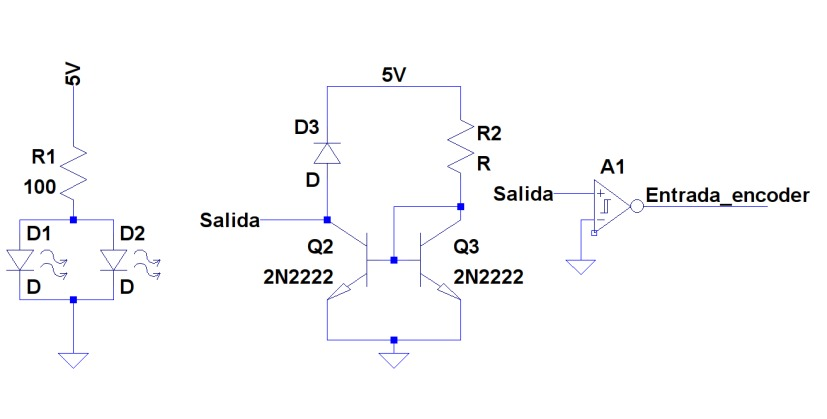
\includegraphics[width=10cm]{./imagenes/circuitoFotodiodo.jpeg}
\caption{circuito del fotodiodo y de los diodos infrarrojos.}
\label{fig:circuitoFotodiodo}
\end{figure}
La señal de salida se conecta a un Schmitt trigger para discretizar la señal y luego la salida de ésta se conecta al microcontrolador. La sensibilidad de los diodos receptores se calibra manualmente por medio de R2.

Los diodos emisores, por su parte, se encuentran conectados en paralelo entre sí y en serie con una resitencia de $100 \Omega$ conectada a la salida de tensión de 5V del kit de desarrollo Arduino Nano. Inicialmente se había diseñado un circuito con espejo de corriente que permitía regular la intensidad de los LEDs desde el microcontrolador para poder adaptarse a cambios de luz en el ambiente, no obstante, las pruebas demostraron que se podía calibrar una intensidad que funcionase bajo todas las condiciones de luz del lugar de trabajo usado, por lo que se descartó el circuito por la simple versión actual.

Se midió con el osciloscopio la señal de salida de la compuerta y se verificó que la misma es una señal cuadrada, modulada por las barras de la jaula de ardilla. Esta modulación, al provenir de un sistema mecánico, copia las asimetrías del sistema por lo que no genera una onda cuadrada perfectamente simétrica mientras se mantiene una velocidad angular constante.

\subsubsection{Medición de Velocidad con el Microcontrolador}
Las señales acondicionadas de los encoders (ver figura \ref{fig:circuitoFotodiodo}) se conectan a entradas del microcontrolador, donde se resuelve la medición de velocidad por medio de interrupciones. Para ello se utilizan pines con interrupción
por cambio de estado y se mide el tiempo entre interrupciones sucesivas. Esta medición de tiempo presenta una serie de problemas explicados a continuación.

El microcontrolador ATmega328P posee un total de 3 timers. El timer1 se utilizó para generar los PWM de los motores, mientras que el timer2 se utilizó para la generación de un tiempo de muestreo constante para el sistema. Esto dejaba únicamente el timer0 disponible para realizar la medición de tiempos entre interrupciones,
sin embargo, dado que el timer0 es el que utilizan las librerías de Arduino por defecto, se decidió buscar una alternativa que permitiese reservar este timer para realizar tareas de depuración. Para ello se decidió utilizar el timer2 de forma simultánea para las interrupciones constantes a Ts (periodo de muestreo) y para el conteo de tiempo.

Para entender cómo usar de forma conjunta el timer, consideremos lo que ocurre cuando se inicia el microcontrolador. Cada vez que el timer2 desborda se incrementa una variable auxiliar $cantOVerflow$. Cuando se detecta el primer cambio de estado o flanco (interrupción por pin), el tiempo transcurrido va a ser:
 \begin{equation*}
 t=\frac{Prescaler}{f_{clk_{io}}} (TCNT2+cantOVerflow\ OCR2A)
 \end{equation*}
Ya que la cantidad de pulsos contados por el timer es igual al valor actual del timer (registro TCNT2 del microcontrolador) más $cantOVerflow$ veces el máximo valor que cuenta (dado por el registro $OCR2A$ del microcontrolador).

Una vez guardado el valor del timer actual, reseteamos $cantOVerflow$. Así, la siguiente vez que se genere una interrupción el valor de $cantOVerflow$ reflejará la cantidad de overflows que hubo desde la interrupción pasada. Si a la siguiente interrupción por cambio de estado de la señal del encoder hacemos el cálculo de tiempo como
antes, tendremos un error de cálculo debido a que en realidad no transcurrieron $cantOVerflow$ ciclos de conteo completos del timer, sino que el primero arrancó a contar desde el valor que tenía el timer cuando se hizo la interrupción anterior. Para eso agregamos una variable auxiliar de corrección cuyo valor sea siempre el valor del
timer al momento de la última interrupción:
 \begin{equation}
 t=\frac{Prescaler}{f_{clk_{io}}} (TCNT2+cantOVerflow\ OCR2A-TCNT2_{anterior})
 \end{equation}

Como este cálculo debe realizarse para cada motor, el código de interrupción por cambio de estado verifica cuál encoder generó la interrupción y almacena las variables necesarias para hacer el cálculo de velocidad del motor ($TCNT2$, $TCNT2anterior$ y $cantOverflow$ para cada motor) en el código principal, es decir, fuera de la interrupción para no consumir tiempo de ejecución con prioridad (interrupción) del microcontrolador.

Conociendo el tiempo entre interrupciones, el cálculo de velocidad correspondiente en rpm se realiza según la fórmula:
\begin{equation*}
\omega=60 \frac{seg}{min}\ \frac{1}{D\ t}
\end{equation*}

Donde $D$ es la cantidad de varillas del encoder. 

%Esto habría que revisarlo... $.$
Para el primer modelo de encoder utilizado la señal cuadrada a la entrada del microcontrolador presentaba variaciones en el ancho del pulso debidas al movimiento de la rueda que se encontraba ligeramente descentrada. Para evitar este inconveniente y las variaciones introducidas por posibles asimetrías en la fabricación del encoder,
se decidió calcular la velocidad con el tiempo demorado en realizar una vuelta entera. Para el modelo de encoder actual esto no debería ser tan necesario, sin embargo se ha mantenido en el código. El resultado de esta forma de medición equivale a agregar un filtro discreto de media movil (moving average). El efecto de esto se verá más
adelante.
Sabiendo que la mínima variación de tiempo está dada por la cantidad de conteos realizados por el timer, resulta evidente que mientras más rápido cambie el timer mayor precisión se tendrá en la medición de velocidad.
Sabemos que el timer genera interrupciones cada:
\begin{equation}
T_{int}=\frac{Prescaler(1+OCR2A)}{f_{clk_{io}}}
\end{equation}
por lo que si se desea un $T_{int}$ pequeño se debe utilizar un prescaler lo menor posible. Dado que este mismo $T_{int}$ es el que se utiliza para generar la frecuencia de muestreo constante, se aumenta el prescaler efectivo para la determinación de $Ts$ utilizando una variable auxiliar como contador. Así, la frecuencia de muestreo del sistema será un múltiplo de $T_{int}$. Para determinar el valor del prescaler a utilizar se debe tener en cuenta que el tiempo $T_{int}$ sea suficiente para realizar las operaciones necesarias en la interrupción por overflow del timer y para que estas interrupciones no se generen con una frecuencia tan alta que impida el correcto funcionamiento de las restantes interrupciones.

\subsection{Sensor de Línea}
Los sensores de línea utilizados regularmente consisten en una serie de fotodiodo y LEDs infrarrojos colocados en dos líneas paralelas. %El mecanismo se detalla a continuación:

Suponga que el sensor se encuentra sobre una superficie reflectante (por ej. de color blanca).
 Luego la luz emitida por el LED IR se reflejará y llegará al fotodiodo con una intensidad $I_{blanco}$.\\
Ahora suponga que el sensor se encuentra sobre una superficie poco reflectante (por ej. de color negra). Luego la luz emitida por el LED IR se reflejará y llegará al fotodiodo con una intensidad $I_{negro}$.\\
Entonces, siempre y cuando la diferencia entre estas intensidades sea mayor que la sensibilidad del sensor  $|I_{blanco} - I_{negro} |> I_{sens}$, se podrá discernir entre una superficie y la otra. \\
Generalmente cuando cambia el color de una superficie también cambia el material de la misma, por lo que no se puede asegurar que \textit{siempre} una superficie de color negro generara una intensidad reflejada menor que una superficie de color blanco $I_{negro} <I_{blanco}$. 
 La idea se muestra en la figura \ref{fig:sensorLinea}.\\
%Completar!! $.$
\begin{figure}[h]
\centering
\includegraphics[width=8cm]{./imagenes/sens_rebotando2.png}%sensorLinea.png
\caption{En esta implementación se ve el cabezal circular con 2 leds emisores. El led Rojo hace las veces de led Emisor de luz y el led Azul como fotodiodo.}
\label{fig:sensorLinea}
\end{figure}
La región en donde se ve la luz de color rojo, es en donde los fotones inciden en la superficie y no son captados por el fotodiodo (led azul), por otro lado la región en donde solo se ve la luz azul es la zona en donde el fotodiodo posee mayor sensibilidad para captar los fotones reflejados y ademas no coincide con la zona de incidencia del LED IR. La superposición de los colores es el intervalo espacial en donde la luz emitida por el led rojo es recibida por el fotodiodo. Esta zona es en donde se evaluara si la zona es muy reflectante o poco reflectante, es decir, si hay una linea o no.
\subsubsection{Circuito Eléctrico}
Para alimentar este arreglo de emisores y receptores se utilizó el circuito de la figura \ref{fig:circuitoSensorLinea}. En ella se observa que los diodos se alimentan a través de espejos de corriente que permiten ajustar la intensidad de luz emitida. La sensibilidad de todos los fotodiodos se ajusta por medio de $R_2$, las salidas se conectan a compuertas Schmitt trigger para acomodar la señal de salida a una que permita trabajar con lógica digital. Se corroboró con el osciloscopio que la señal de salida era apropiada para la lectura digital por parte del microcontrolador.
\begin{figure}[h]
	\centering
	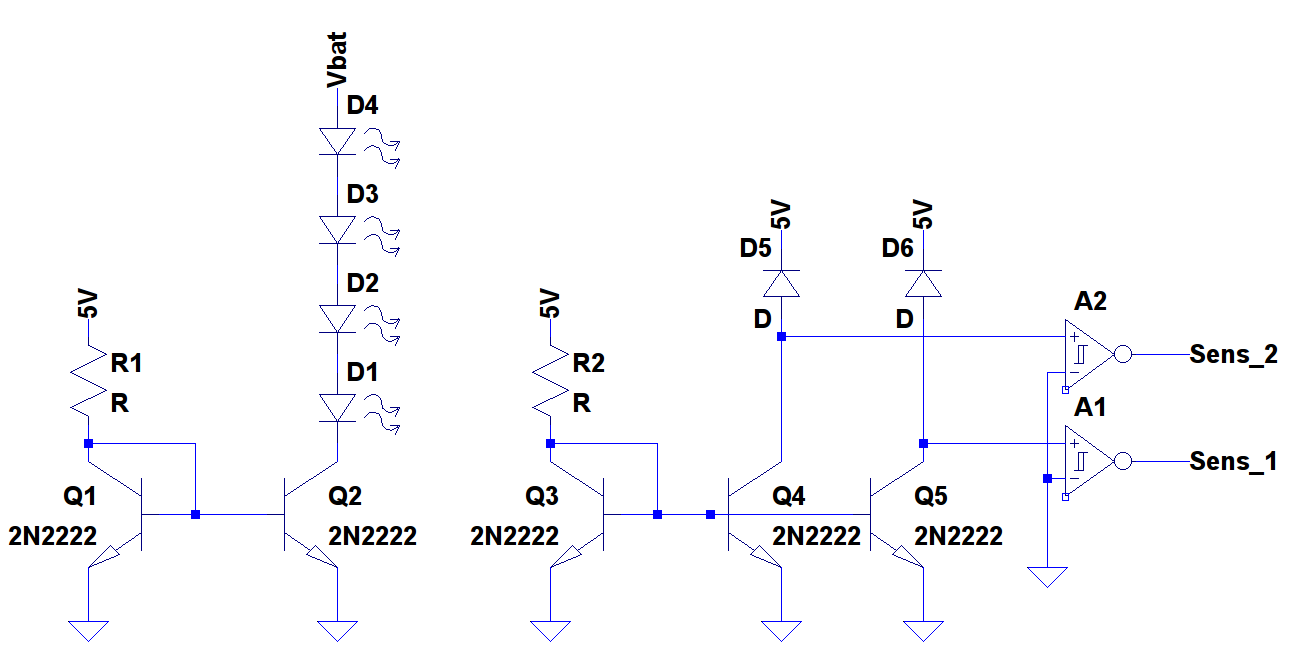
\includegraphics[width=10cm]{./imagenes/circ_sens_lin.png}%circuitoSensorLinea
	\caption{circuito utilizado para alimentar los diodos LED infrarrojos y los correspondientes fotodiodos que componen el sensor de línea. Este esquema permite ampliar la cantidad de sensores a la que se desee. En el dispositivo final se cuenta con 8 fotodiodos. }
	\label{fig:circuitoSensorLinea}
\end{figure}

\subsubsection{Estructura Mecánica}
La disposición física de los LEDs estaba dada inicialmente por la placa PCB utilizada en el circuito. Esto hacía que los LEDs se encontraran a alturas ligeramente variables y con leves diferencias de inclinación, además de que la placa no se encontraba centrada respecto al cuerpo del robot por estar colocada en una posición
casi arbitraria. A pesar de estos problemas, el sensor presentaba un desempeño básico aceptable que permitió realizar las pruebas necesarias hasta lograr que el robot realizara el seguimiento de una pista. No obstante, una vez finalizado el prototipo inicial, se rediseñó la estructura para solucionar estos problemas. En esta etapa
del trabajo se diseñaron y fabricaron dos estructuras alternativas: la primera con una disposición de los LEDs  lineal y la segunda con una disposición circular. Esta última se propuso en función del análisis realizado en la sección Modelado del Sistema [\ref{sec:Modelado_del_sistema}], según el cual podíamos trabajar con un modelo LTI simple
si considerábamos únicamente el ángulo de desviación de la orientación del robot respecto de la línea. Las estructuras obtenidas pueden observarse en la figura \ref{fig:estructuraSensor}. 
\begin{figure}[h!]%!: Override internal parameters LaTeX uses for determining "good" float positions.
    \centering
    \begin{subfigure}[h]{0.45\textwidth}
    	\centering
        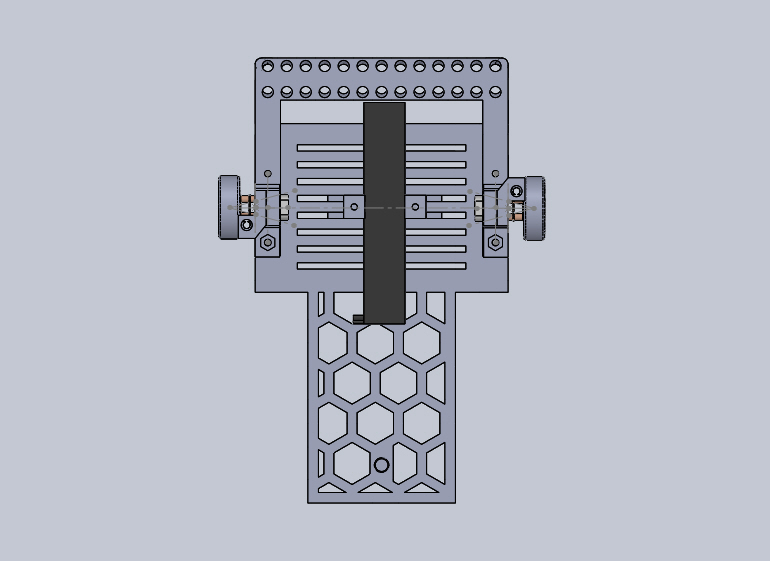
\includegraphics[width=7.5cm]{./imagenes/conSensorLineal.png}
        \caption{}
    \end{subfigure}
    \quad
    \begin{subfigure}[h]{0.45\textwidth}
    	\centering
        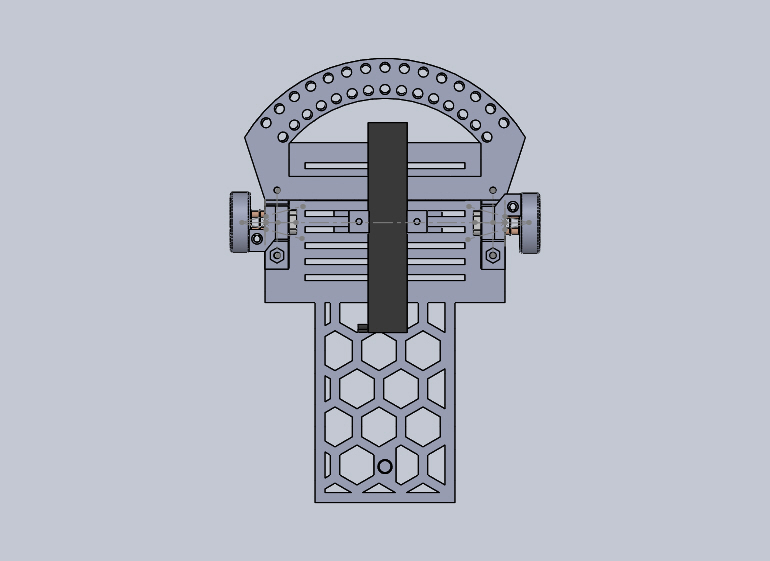
\includegraphics[width=7.5cm]{./imagenes/conSensorCircular.png}
        \caption{}
    \end{subfigure}
    \caption{esquema del robot con los dos tipos de estructuras diseñadas para fijar la disposición de los diodos según la configuración geométrica deseada: (a) lineal, y (b) circular.}
	\label{fig:estructuraSensor}
\end{figure}

Se optó por diseñar las dos variantes para poder probar a futuro distintas estrategias de control, no obstante, la utilizada actualmente funcionaría mejor con la disposición circular. Además, para permitir variar las pruebas en etapas de desarrollo, se diseñaron las estructuras con agujeros adicionales para tener la posibilidad de agregar LEDs o modificar la distancia entre los mismos. Para las pruebas mostradas en este informe se utilizó una configuración con 8 pares de LEDs ubicados desde los extremos al centro dejando un lugar vacío entre ellos.
\subsubsection{Valores de Lectura}
Considerando que se deseaba obtener un valor de ángulo como lectura del sensor, se podría haber realizado una deducción geométrica de los valores de ángulo a asignar para cada lectura posible del sensor. Sin embargo, dado que el diseño inicial tenía múltiples asimetrías, que resultaba difícil identificar correctamente el centro del robot y que los diodos utilizados pueden presentar imperfecciones o diferencias de sensibilidad, se optó por realizar un ensayo donde se midiera el rango de valores de ángulo de desviación para el cual se mantenía cada medición posible del sensor. Este ensayo se realizó marcando en un papel líneas de referencia y colocando cinta en línea recta sobre el mismo. Girando el robot sobre la pista con el centro siempre sobre un punto medio de la línea, se marcaron los rangos de desviación para los cuales se mantenía cada medición del sensor.
\subsubsection{Lectura del Sensor con el Microcontrolador}
Las salidas de las compuertas se conectan a pines de entrada del microcontrolador. En el programa principal la medición de la línea se necesita cada vez que se calcula el PID del sistema total, por ello se programó una subrutina de medición que se llama en el programa principal (main) antes de calcular el controlador cada $Ts$ segundos. Dentro de esta subrutina se lee cada valor digital de entrada y se almacenan los resultados en un vector de 8 componentes. Para anticiparse a valores de mediciones atípicos y atenuar el efecto de posibles errores de medición, se calcula una suma ponderada de las entradas para obtener un número que indica debajo de cuál de los fotodiodos se encuentra el centro de la línea, siendo las posibilidades para el caso de 8 LEDs: $1, 1.5, 2, 2.5,...,7,7.5$ y $8$, donde los números no enteros representan el caso en el que la línea se encuentre entre dos fotodiodos. Si a este número lo multiplicamos por dos y le restamos dos, nos queda uno de los siguientes resultados: $0,1,2,...14$, que pueden usarse como índice de un vector. De esta forma lo que se hace es definir un vector constante con los resultados de ángulo obtenidos por ensayo cuando la línea estaba bajo cada una de las posibilidades y utilizar el número calculado para definir con cuál de los elementos del vector quedarse como medición actual. El caso en que todos
las entradas estén en $0$ se toma como valor particular y se la asigna el número 3 para que funcione como bandera e indique que se perdió la línea. Cuando esto ocurre el programa principal mantiene para los cálculos el último valor válido medido.

\section{Identificación de Sistemas}
\label{sec:identifSist}
Para sintonizar los controladores PID ha implementar se necesita tener algún tipo de información sobre el comportamiento de la planta a controlar. En función de lo definido en la sección \ref{sec:estrategia_de_control}, las plantas a identificar o caracterizar son tres: los dos motores, cuyo modelado matemático se analizó en la sección \ref{modeloMotores}, y el sistema total, que incluye los motores con sus PID y la cinemática del robot analizada en la sección \ref{modelo cinematico}.

A continuación se detallan los ensayos realizados para la identificación de los sistemas a controlar.
\subsection{Identificación de los Motores}
El modelo de función de transferencia planteado matemáticamente en la sección \ref{modeloMotores} define como variable de salida la velocidad angular del motor $\omega $ y como variable de entrada la tensión promedio aplicada entre sus bornes. Para la implementación con el microcontrolador se utiliza una señal de PWM de alta frecuencia (comparada con la frecuencia de corte del polo mecánico y el polo eléctrico) cuyo duty cycle modifica el valor de tensión continua aplicado al motor. Esto es factible debido a que el \textit{ sistema motor} actúa como un filtro pasabajos, manteniendo la componente de continua de la señal y atenuando las restantes. Dado que esta es la señal que se puede controlar realmente, se utiliza como señal de entrada el duty cycle utilizado en los PWM.

El modelo obtenido de forma teórica realiza varias simplificaciones. Una de ellas es ignorar el ciclo de histéresis de los motores y otra es no considerar el efecto de una carga en el motor, que en este caso implicaría considerar la dinámica del robot sobre el suelo. Estos fenómenos hacen que el comportamiento real de los motores no sea realmente lineal. Para analizar la linealidad el sistema y el intervalo de trabajo a utilizar se diseñó un ensayo que barriera las distintas posibilidades de duty cycle para cada motor y almacenara varias muestras de las velocidades obtenidas en el estado estacionario. En la figura \ref{linealidad} se muestra la curva obtenida para el motor B. La del motor A es análoga. %$.$ Revisar que ya esté explicado en algún lado que el motor B es el derecho y el A el izquierdo

%$.$ Está mal el eje Y! Corregir imagen
\begin{figure}[h]
\centering
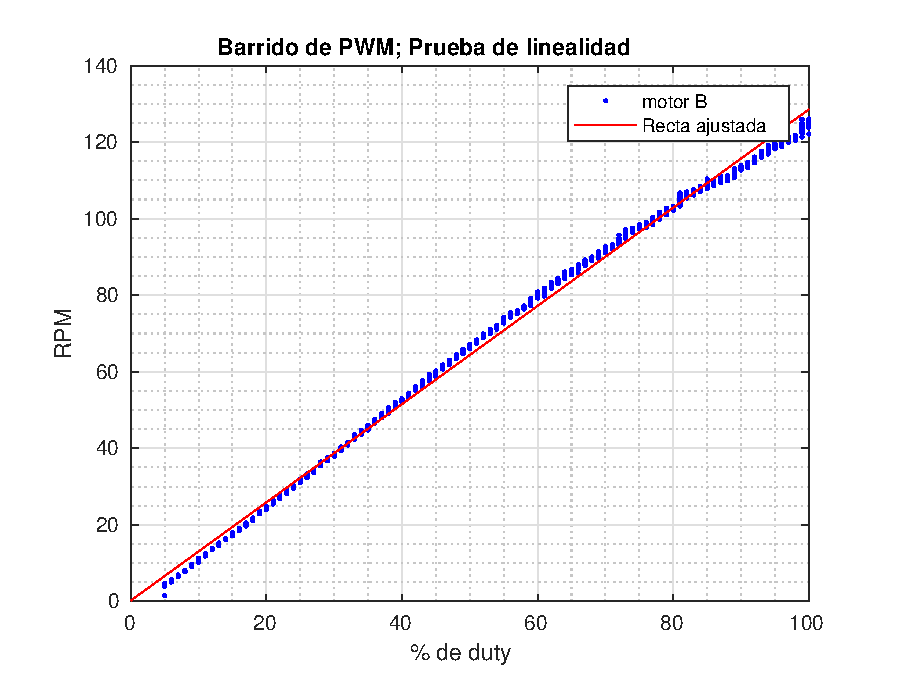
\includegraphics[width=10cm]{./imagenes/prueba_linealidad.eps}
\caption{Curva de respuesta entrada-salida para el motor B.}
\label{linealidad}
\end{figure}

Analizando la curva de respuesta del sistema observamos que los motores comienzan a moverse recién a partir de un 5\% de duty cycle. Esto se debe al par de fricción estática aplicada al eje. Por otra parte, la recta ajustada muestra que el comportamiento es aproximadamente lineal hasta un 80\% de duty cycle. Para garantizar un buen funcionamiento se trabajará de $10\%$ a $80\%$ para los ensayos de estimación del sistema.

En función de las consideraciones anteriores, se diseño un ensayo que permitiese obtener la respuesta al escalón de ambos motores. Dado que es de interés conocer el comportamiento con carga y no en vacío, se buscó que el ensayo se realizara con el robot completo funcionando en condiciones normales. Para ello se programó que el robot anduviera en línea recta, primero a una velocidad baja y luego a una mayor dada por un cambio repentino del duty cycle de ambos motores. Las señales de interés se muestrearon a una frecuencia de 200Hz, se almacenaron en la EEPROM y luego fueron transmitidas a la computadora por puerto serie. La curva obtenida de ambos motores se muestra en la figura \ref{EscalonMotores}.
\begin{figure}[h]
\centering
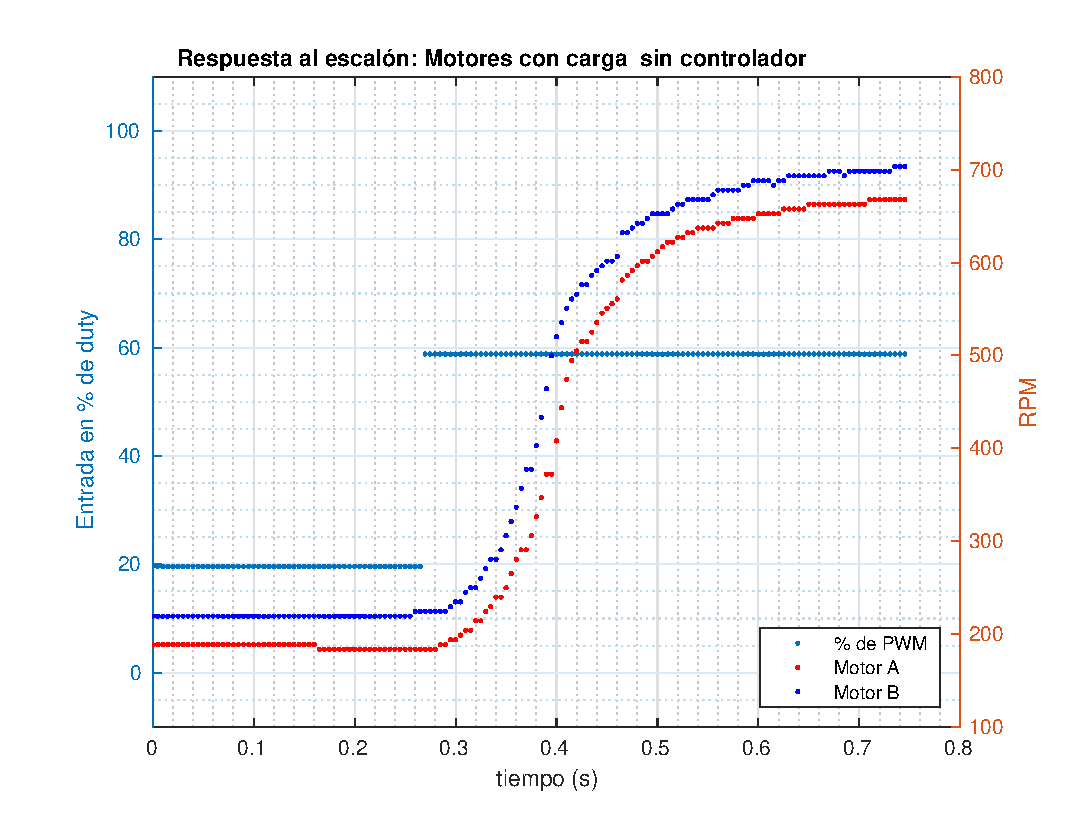
\includegraphics[width=10cm]{./imagenes/resp_escalon_motores_2}
\caption{Respuesta al escalón de ambos motores a lazo abierto con carga.}
\label{EscalonMotores}
\end{figure}

Analizando los resultados obtenidos se detectó que existía una demora en el sistema no anticipada por el modelo matemático. Ésta se debe a la dinámica del sistema de medición de velocidad, que en los análisis teóricos no se suele considerar. Específicamente, el promedio realizado al momento de medir la velocidad de cada motor genera la demora observada. Dado que se almacenan los tiempos correspondientes a un giro completo de la rueda  para realizar el cálculo de velocidad, cuando la velocidad real cambia de forma abrupta el sistema demora una revolución del eje en reemplazar todas las mediciones y por lo tanto en otorgar una medición confiable. Este comportamiento se corresponde con el de un sistema de media móvil, pero variante en el tiempo y alineal, ya que la demora depende de la velocidad de giro. Para poder continuar trabajando en el contexto de sistemas LTI se utilizará una estimación del sistema alrededor de cierto punto de trabajo. 

Utilizando los datos obtenidos se estimó un sistema LTI continuo mas un retardo tal que se ajuste a cada curva utilizando la herramienta de Matlab System Identification \cite{Sys_ident}. Las funciones de transferencias obtenidas, fueron ajustadas con un $ 95.15\%$ para el motor A y $ 96.65\%$ para el motor B. Las mismas se muestras a continuación:
\begin{equation}
M_a(s)= \frac{7075.3 e^{-0.013s}}{(s+9.631)(s+67.5)}
\end{equation}
\begin{equation}
M_b(s)= \frac{5042.1 e^{-0.013s}}{(s+9.988) (s+45.48)}
\end{equation}

Cabe aclarar que la precisión del ajuste depende mayoritariamente de como fueron tomadas las muestras. En este caso la metodología de medición genera un delay variable con las $RPM$ (mayor delay a bajas $RPM$), por lo que se optó por ajustar los modelos para un ensayo escalón en el cual se producirá el mayor delay. 
%$.$ Utilizando esta información se ajustaron los controladores PID de cada motor, según se explicará en la sección \ref{control}. 
\subsection{Identificación de la Cinemática el Robot}
En función de lo analizado en la sección \ref{modelo cinematico}, podemos pensar que si el robot arranca alineado con una línea recta, y manteniendo la restricción de $v$ constante, entonces la planta se comporta como un sistema cuya entrada es $\Delta \omega$ y su salida $\theta$, gobernado por la ecuación \ref{eq:tita_omega}. Para un mayor entendimiento se reemplaza $\theta$ por $\beta$ ya que si bien $\theta \approx \beta $ cuando $|Y_0| \approx 0$, no es válido en todo momento. Bejo esta justificación la ecuación se escribe de otra manera a continuación 

\begin{equation}
\dot{\beta}= \frac{r\Delta\omega}{L} 
\label{eq:sys_tot_teo} 
\end{equation}

Para realizar el ensayo al escalón se debería empezar con $\Delta \omega = \beta = 0$  y luego cambiar $\Delta \omega$  abruptamente a un valor final, midiendo el valor de $\beta$ obtenido. Físicamente esto implica que el robot debe empezar andando a velocidad constante, perfectamente alineado con la línea, y luego girar hasta perder la línea (más allá de este punto no tiene sentido seguir porque se pierde la medición).
Si el cambio de velocidad de los motores fuese automático, el robot giraría siguiendo una circunferencia perfecta como se ve a en la figura \ref{fig:carritoEsc}.
\begin{figure}[h!]
\centering
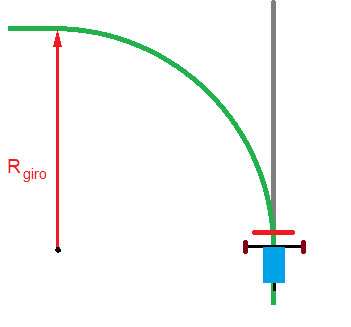
\includegraphics[width=6cm]{./imagenes/carrito_Ensayo_escalon.png}
\caption{Trayectoria seguida por el robot si empieza a girar a $\Delta \omega $ constante (verde) arrancando inicialmente alineado con la línea (gris).}
\label{fig:carritoEsc}
\end{figure}
%Lo que nos interesa es saber cuánto tiempo transcurre hasta que pierde la línea. Dicho punto sería cuando el último sensor de la derecha está sobre la línea verde. Si la distancia entre el eje central del robot y éste LED es $d_1$, entonces el LED se desplaza siguiendo una trayectoria circular de radio $R_{giro}$+$d_1$ …..

Sin embargo, la implementación perfecta de un ensayo al escalón resulta muy difícil por dos inconvenientes. El primero es que se requiere que durante un tiempo el robot siga la línea perfectamente antes de girar. Para lograr esto se implementó un controlador proporcional ajustado a mano que permitía que el robot siga la pista. Así, el código implementado sigue la línea usando este controlador durante un breve lapso de tiempo que permita la estabilización del robot y luego desactiva el controlador y cambia abruptamente la diferencia de velocidad de los motores (manteniendo $v$ constante), siendo los valores del ensayo los tomados a partir de este instante de tiempo.
El segundo conflicto es que la señal que realmente se puede controlar no es la diferencia real de velocidad de los motores, sino la diferencia de velocidad deseada. La diferencia entre ambas señales está dada por la dinámica de los motores con sus controladores correspondientes. Como sólo se desea estimar la sección correspondiente a la cinemática, se optó por medir las señales de entrada y salida de esta sección, es decir, $\Delta \omega$ real y $\beta$, y utilizar esas señales para estimación con el System Identification de Matlab \cite{Sys_ident} . %{\color{red}De esta manera, no se tiene exactamente la respuesta al escalón, pero la señal es lo suficientemente parecida como para resultar de utilidad en la estimación.}

En la figura \ref{fig:ensayoSistTotal} se muestra uno de los resultados de este ensayo.
\begin{figure}
\centering
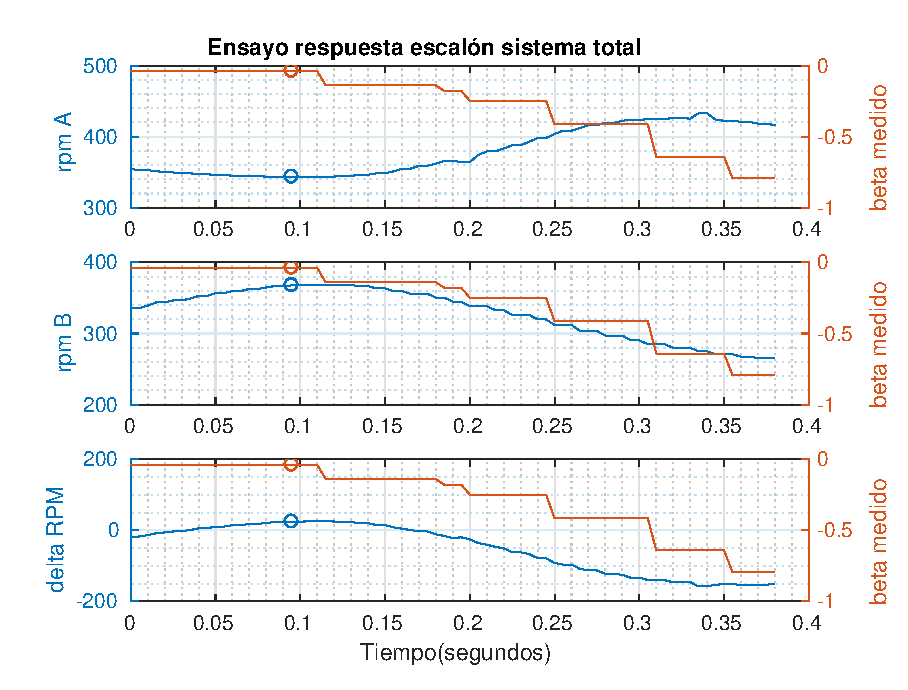
\includegraphics[width=10cm]{./imagenes/resp_escalon_sys_total}
\caption{Resultado del ensayo de respuesta al escalón del sistema total. El circulo marca cuando se desactiva el control y el sistema comienza a trabajar en lazo abierto. En esta caso $\Delta \omega=-50 $ RPM}
\label{fig:ensayoSistTotal}
\end{figure}
Utilizando un conjunto de estos ensayos se estimó el siguiente sistema
\begin{equation}
Sys_{tot}= \frac{0.028934}{s}  
\label{eq:sys_tot_est}
\end{equation}
el cual explica un $82.93\%$ de los datos utilizados en el mejor de los casos.


De la ecuación \ref{eq:sys_tot_teo} y de \ref{eq:sys_tot_est}  se concluye que $\frac{r}{L}=0.028934 $. Los parámetros medidos, si embargo, son $r=1.5cm$ y $L=16cm$, lo cual daría $\frac{r}{L}=0.09375 $. Esta discrepancia no se pudo explicar aún.   
%$.$ Faltaría una imagen que muestre qué tan bien ajusta el modelo estimado.

\section{Ajuste de los Controladores} 
\subsection{Control Motores}
\label{sec:ajus_control}
Existen diversas estrategias para realizar la sintonización de un controlador PID. Una de las posibilidades estudiadas en la carrera es la utilización de tablas empíricas, como son los métodos de Ziegler Nichols. Inicialmente se quiso implementar el ajuste con uno de estos métodos por considerárselo más didáctico y porque no requiere un modelo completo de la planta. Más adelante se detalla el procedimiento seguido, no obstante los controladores obtenidos no presentaban un desempeño satisfactorio.

Otras opciones estudiadas en la carrera requieren disponer de un modelo completo del sistema a controlar. Es por esto que se realizaron las estimaciones de funciones de transferencia explicadas en la sección \ref{sec:identifSist}. Conocidos los modelos de los sistemas, se puede realizar un ajuste con fundamentos matemáticos, pero dado que resulta más rápido y más intuitivo se optó por realizar un ajuste por software. Para ello se usó la herramienta de PID tuner de Matlab \cite{PID_tuner} que permite un ajuste muy fácil observando la curva de salida. Esto resulta de gran utilidad ya que se puede ver en la gráfica el impacto en el comportamiento efectivo, mientras que los cálculos teóricos estudiados en la carrera utilizan restricciones sobre los parámetros matemáticos que se relacionan de forma indirecta, aproximada y menos tangible con la respuesta temporal que realmente tendrá el sistema a lazo cerrado.

Para el ajuste de los controladores de los motores se buscó que la respuesta al escalón fuese rápida y con poco sobreimpulso, ya que el impacto se vería incrementado al considerar todo el robot en su conjunto. Además, se buscó un ajuste que diera un comportamiento muy similar para ambos motores, ya que las asimetrías se traducirían en trayectorias erráticas. Los controladores obtenidos para cada motor fueron los siguientes:
\begin{equation*}
C_a(s)= \frac{  19.243 (s-11.74)}{s}
\end{equation*}
\begin{equation*}
C_b(s)= \frac{ 18.68 (s-10.93)}{s}
\end{equation*}

El ajuste se realizó en tiempo continuo, con lo cual resulta necesario realizar una discretización del controlador para poder implementarlo en el microcontrolador. La discretización utilizada fue la de Backward Euler (o diferencias hacia atras).
%, la cual realiza la siguiente sustitución:
%\begin{equation*}
%s=\frac{z-1}{zh}
%\end{equation*}%$.$ esto no sé si queda bien así
%$.$ No me acuerdo qué era lo que hacíamos inicialmente que daba unos coeficientes enormes. Eso hay que ponerlo

Una vez implementados los controladores, se repitió el ensayo al escalón con el sistema a lazo cerrado. El resultado es el mostrado en la figura \ref{fig:respEscLazoCerrado}.
\begin{figure}[h]
\centering
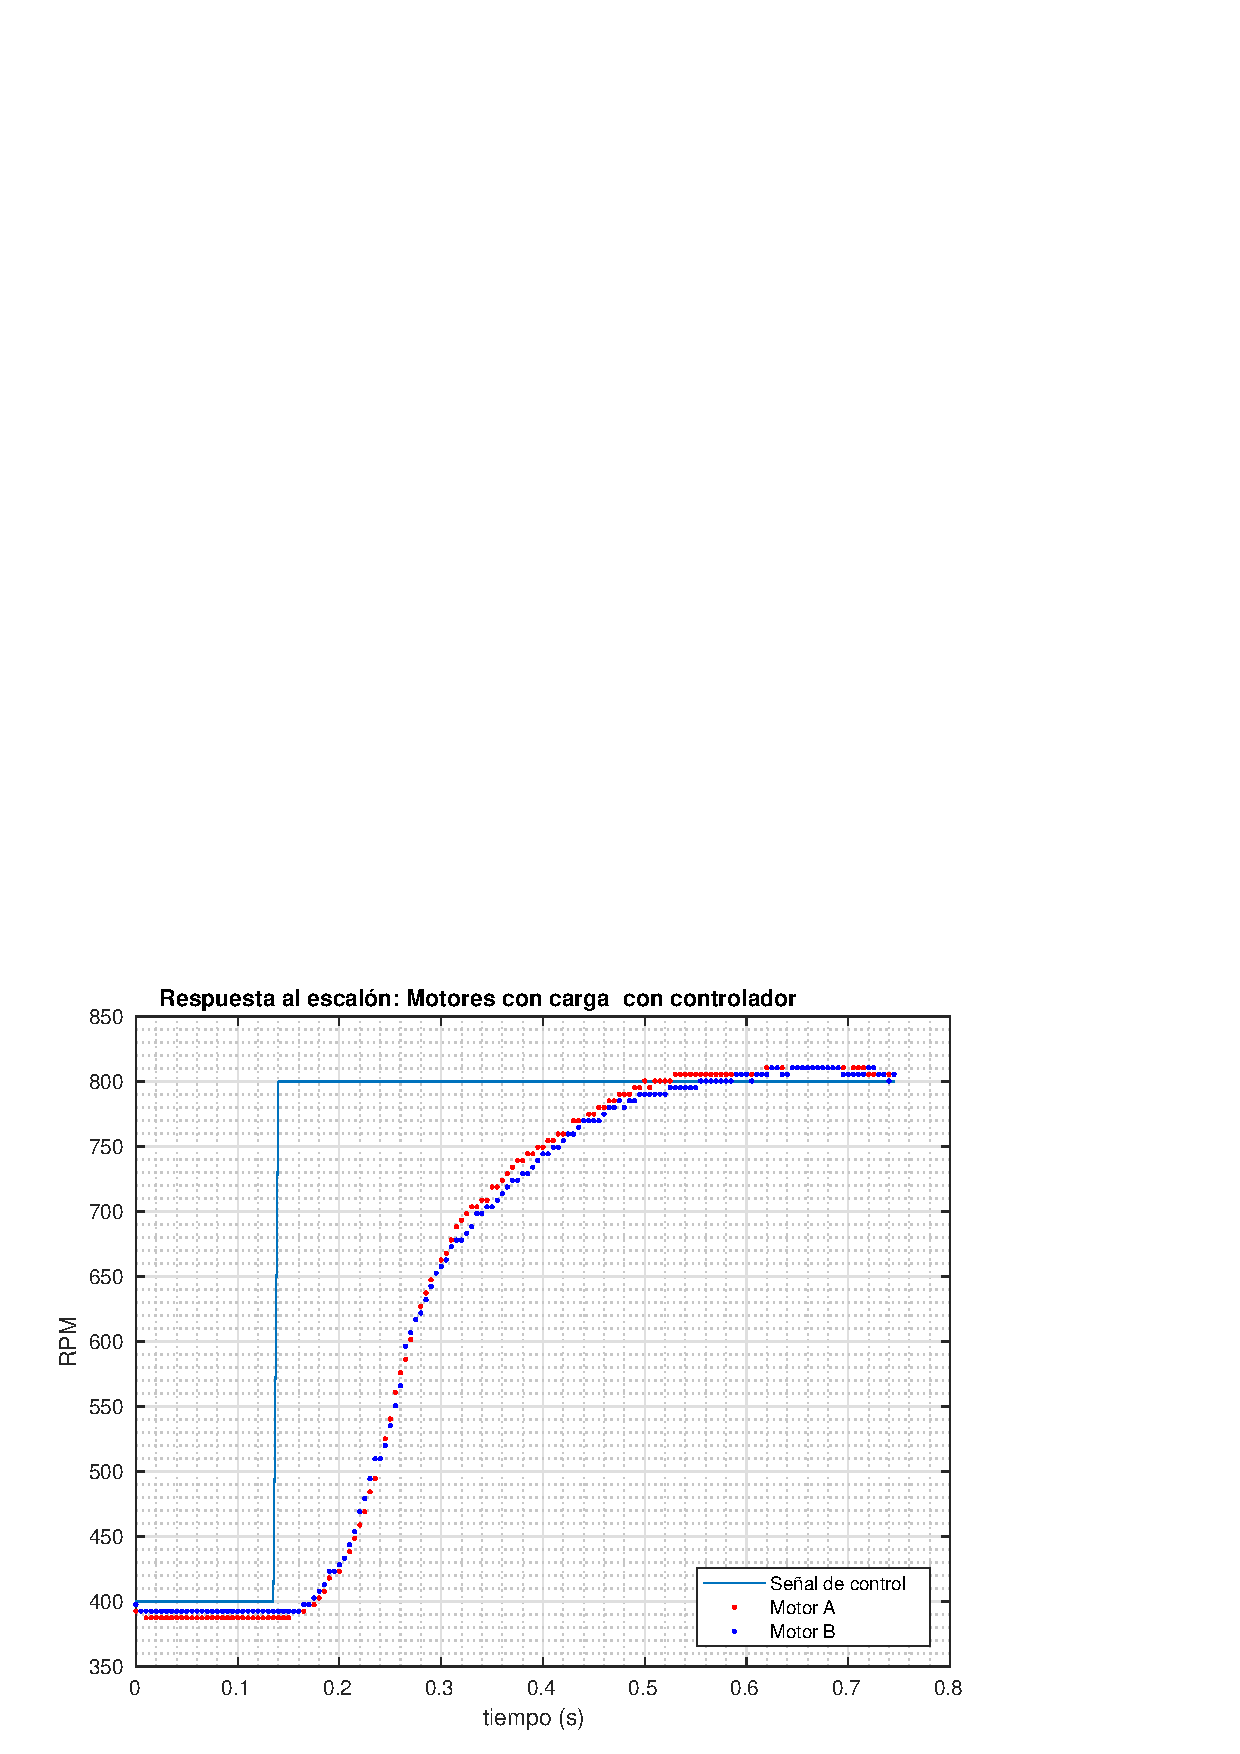
\includegraphics[width=10cm]{./imagenes/resp_escalon_motores_controlados_2}
\caption{Resultado del ensayo de respuesta al escalón para ambos motores funcionando con los controladores PI calculados.}
\label{fig:respEscLazoCerrado}
\end{figure}
Se observa que se pudo alcanzar el objetivo propuesto de reducir la asimetría de los motores.

\subsection{Sintonizacion de controlador PID mediante reglas de Ziegler Nichols} %$.$ no lo leí
%Explicar que es un controlador PID antes. Lo que sigue es un choreo del ogata\\

Según \cite{ogata} casi todos los controladores PID se ajustan en el sitio, en la literatura se han propuesto muchos tipos diferentes de reglas de sintonización, que permiten llevar a cabo una sintonización delicada y fina de los controladores PID en el sitio. Asimismo, se han desarrollado métodos automáticos de sintonización y algunos de los controladores PID poseen capacidad de sintonización automática en línea. Actualmente se usan en la industria formas modificadas del control PID, tales como el control I-PD y el control PID con dos grados de libertad.

La utilidad de los controles PID estriba en que se aplican en forma casi general a la mayoría de los sistemas de control. En particular, cuando el modelo matemático de la planta no se conoce y, por lo tanto, no se pueden emplear métodos de diseño analíticos, es cuando los controles PID resultan más útiles. En el campo de los sistemas para control de procesos, es un hecho bien conocido que los esquemas de control PID básicos y modificados han demostrado su utilidad para aportar un control satisfactorio, aunque tal vez en muchas situaciones específicas no aporten un control óptimo.

Las reglas de Ziegler-Nichols son muy convenientes cuando no se conocen los modelos matemáticos de las plantas. Tales reglas sugieren un conjunto de valores de $K_p$, $T_i$ y $T_d$ que darán una operación estable del sistema. No obstante, el sistema resultante puede presentar una gran sobreelongación en su respuesta escalón de forma que resulte no aceptable. En tales casos se necesitará una serie de ajustes finos hasta que se obtenga el resultado deseado. De hecho, las reglas de sintonía de Ziegler-Nichols dan una estimación razonable de los parámetros del controlador y proporcionan un punto de partida para una sintonía fina, en lugar de dar los parámetros $K_p$, $T_i$ y $T_d$ en un único intento.

Tal determinación de los parámetros de los controladores PID o sintonía de controladores PID se pueden realizar mediante experimentos sobre la planta. Hay dos métodos denominados reglas de sintonía de Ziegler-Nichols: método de la respuesta al esalón y método del $K_{inestable}$. En este trabajo se implemento el primero, por lo que sólo se detallara ese. En caso de querer profundizar mas en el tema, puede consultar \cite{biblia_PID} \cite{paginaPID}. 

\subsubsection{Metodo de Z-N: respuesta al escalón}
%Esto esta sacado del PDF que nos paso COLON:\\

Según \cite{biblia_PID} este método se basa en registrar la respuesta a un escalón
unitario del sistema a lazo abierto, para luego ajustar los tres parámetros de un modelo
de primer orden con retardo dado por la ecuación \ref{eq:ajusteZN}.

\begin{equation}
G_s(s)=\frac{K_p}{Ts+1}e^{-sL}
\label{eq:ajusteZN}
\end{equation}


\begin{figure}[h]
\centering
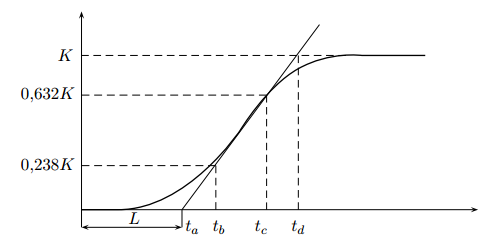
\includegraphics[width=10cm]{./imagenes/escalon_z-n.png}
\caption{Determinación gráfica de los parámetros de un modelo a partir de
la respuesta escalón en forma de S}
\label{fig:escalon_zn}
\end{figure}




Los parámetros del modelo de la ecuación \ref{eq:ajusteZN} pueden ser determinados por medio de la figura \ref{fig:escalon_zn}. La ganancia estática $K$ la obtenemos del valor final de la salida del proceso dividido el valor máximo de la entrada. 

Para hallar los otros dos parámetros hay varias alternativas. Una de ellas consiste en trazar una recta tangente al punto donde de la respuesta al escalón presenta la mayor pendiente. El valor de la demora $L$ lo obtenemos de la intersección de esta recta con el eje horizontal. El valor de la constante de tiempo $T$ lo podemos obtener a partir de la distancia $t_a-t_c $, donde $t_c$ es el tiempo donde la respuesta al escalón es $0.632K$.
Otro método, un poco más preciso, consiste en determinar los puntos $t_b$ y $t_c$ donde $s(t)$ toma los valores $0.283K$ y $0.632K$, respectivamente. Luego, la demora y la constante de tiempo la hallamos a partir de la ecuación \ref{eq:calculo_T_L}.

\begin{equation}
T=1.5(t_c -t_b) \quad	L=t_c-T
\label{eq:calculo_T_L}
\end{equation}

Como se menciono en la sección \ref{sec:ajus_control} este método no genero resultados satisfactorios en lo que el control de los motores respecta. Una de las causas reside en que este método es valido dentro de un rango de validez \cite[pág. 60]{biblia_PID} dado por $0.1<L/T<1$. Para el caso que nos acomete, dado por el delay de medición, el parámetro $L/T$ oscilaba entre 10 y 6, es decir $L/T \in (6,10) $. 
\subsection{Control de la Orientación - Sistema Total.}

Para el ajuste de este controlador hay considerar la planta completa a lazo abierto, la cual luego de algunas hipótesis se demuestra en la ecuación \ref{eq:sys_tot_LA}. Por comodidad se vuelve a  muestrar a continuación

\begin{equation*}
\frac{\theta(s)}{\Delta \omega}=Sys_O(s)Sys_{MAc}(s)=Sys_O(s)\frac{C_a(s)M_a(s)}{1+C_a(s)M_a(s)}
\end{equation*}
en donde $C_a(s)$ y $M_a(s)$ son el controlador del motor a y el modelo del motor a respectivamente.
Como se detallo en las sección \ref{sec:modelo_orien} llegando a la ecuación \ref{eq:tita_omega}  y se demostró por medio de mediciones que el modelo es \ref{eq:sys_tot_est}, resulta que el sistema de la orientación es un integrador con un polo en el origen. Por la naturaleza del problema, no es viable ajustar un controlador mediante las reglas de Ziegler-Nichol. Además no es realista solo ajustar la parte del control de la orientación de manera independiente del resto del sistema, ya que no se estarían considerando la respuesta de los motores reales ni el sistema completo. Teniendo en cuenta todo esto el procedimiento fue obtener los controladores de los motores, controlar ese subsistema y obtener un modelo de este sistema controlado. El sistema controlado para el motor A resulta

\begin{equation}
Sys_{MAc}(s)=\frac{C_a(s)M_a(s)}{1+C_a(s)M_a(s)}
\end{equation}    

lo cual si se reemplaza por sus valores reales y realizando un poco de algebra se obtiene

\begin{equation}
Sys_{MAc}(s)=\frac{367.68(s+11.74)}{(s+61.79) (s^2 + 15.34s + 69.87)}
\end{equation}

luego considerando el modelo estimado de la orientación del vehículo el sistema a controlar resulta:
\begin{equation}
\frac{\theta(s)}{\Delta \omega(s)}=Sys_O(s)Sys_{MAc}(s)=\frac{10.639 (s+11.74)}{s (s+61.79) (s^2 + 15.34s + 69.87)}
\end{equation}

Con estos resultados se ensayan distintos controladores sobre esta planta con el fin de calificar su rendimiento.


\section{Funcionamiento del Sistema Total}
 \subsection{Resultados} 
\label{sec:resultados}
%Acá iría el resultado de poner el bichito a seguir la pista.

\begin{table}[h]
\begin{center}
\begin{tabular}{|c|c|c|c|c|c|c|c|c|c|}
\hline
Controlador & $E_c [RPM]$ & $T_{as}[s]$ & $N^o$ v &$\omega_{ref}[RPM]$& $\omega_{med}[RPM]$ & $P_l$ & $TV_{med}[s]$ & $\sigma^2_\beta$ &$\Delta\omega _{max} $  \\
\hline \hline
P&466&1.8&4&400&393.012&si&6.315&&443.1373\\ \hline
PI&466&1.85&4&400&392.3911&si&6.135&&376.47\\ \hline
PDF&477&0.88&4&400&392.7832&si&6.5475&&231.3725\\ \hline
PIDF&618&0.784&5&400&393.7146&no&6.006&&325.4902\\ \hline
PIDF&910&0.466&5&500&491.4325&no&5.0586&&360.78\\ \hline

\end{tabular}
\caption{Mediciones de distintos controladores sobre la pista de la facultad. Referencias: $E_c$ esfuerzo del controlador, $T_{as}$ tiempo de asentamiento, $P_l$ pierde pista, $TV_{med}$ promedio de tiempo por vuelta}
\label{tabla:mediciones}
\end{center}
\end{table}

Si bien estos son algunos parámetros que se midieron en los ensayos, quizás existan otras variables mas reveladoras acerca del comportamiento deseado, por ejemplo numero de oscilaciones, estabilidad, entre otras.

Un ensayo implementado se puede ver en este \href{https://youtu.be/hJU_oneTO20}{\underline{VIDEO}}. Corresponde a una prueba con el último controlador PIDF funcionando a $550RPM$, lo cual determina una velocidad promedio de $0.5m/s$. A esta velocidad y sobre la pista, el vehículo no puede completar la prueba de 4 vueltas ya que se sale de la pista antes. 



\section{Conclusiones}
\label{sec:conclusiones}
En función de los objetivos propuestos, se puede asegurar que se logro desarrollar e implementar un robot seguidor de linea basado en componentes fácilmente conseguibles y/o fabricables, lo cual impulsa el desarrollo de esta clase de dispositivos en la institución. 

Se logro implementar todo el sistema en un microcontrolador de bajas prestaciones. El mismo cumple con los requisitos de fácil implementación, amplia documentación, bajos costos, entre otros.  

Se obtuvo por medio de ensayos, los modelos de los motores, se implemento con éxito un controlador PI en cada motor. No se pudo estimar correctamente la planta total ni se obtuvo un modelo del sistema aceptable para alcanzar los requisitos de competición, sin embargo, el dispositivo puede seguir una curva de radio $r=40cm$ a una velocidad de $500RPM$, esto es aproximadamente $47cm/s$ . La herramienta principal utilizada fueron los toolbox de matlab \cite{Sys_ident,PID_tuner}.



Gracias al sistema ABP, se genero la necesidad y motivación de entender en un sentido amplio  la teoría de control clásica, moderna y digital vista a través de las 3 materias curriculares de la carrera. Se hizo énfasis en la implementación de un sistema de control de tiempo discreto ajustado por métodos estandarizados, de tal manera que sean repetibles. El enfrentamiento a distinta clase de problemas garantizo el conocimiento integro de los sistemas de control implementados. % CHAMUYOOOOOOOOOOOOOOOOOOOOOOOOOO 
 
Los modelos de las piezas para imprimir, los circuitos, las placas y el programa se encuentran en esta dirección \href{https://github.com/Seba-san/Trabajo_Final_Controlados/}{\underline{LINK}}.

  


\section{Mejoras a futuro}
Una de las principales trabas en el desarrollo de este proyecto fue el diseño del sistema de medición de velocidad de las ruedas. El método actual, si bien es funcional, posee la desventaja de incorporar un atraso en las mediciones, lo cual limita la rapidez del controlador. Como mejora en este campo se propone implementar medición de la contra fem del motor o determinar un método libre de distorsiones debido al ensamble. Quizás sea viable diseñar un filtro digital que estime la velocidad de las ruedas sin incorporar un atraso considerable. 

Otra limitación observada a la hora de probar distintos controladores, es la resolución del sensor de linea. Como se en los ensayos, los datos del sensor de linea son digitales, por lo que poseen valores discretos a la salida, lo cual limita las capacidades del control para tomar acciones de corrección.

Una última posible mejora es obtener el modelo del sistema con hipótesis mas suaves de las que se utilizaron en esta oportunidad, de forma que el control implementado pueda resolver situaciones en donde la velocidad media del robot sea mayor. Considerar que actualmente las capacidades del dispositivo no se encuentran completamente explotadas, dando margen a una mejora de tiempos y estabilidad en la pista. %potencia total utilizada de todo el dispositivo % ronda un $40\%$ de su capacidad total, se estima que el rendimiento en pista puede mejorar sus tiempos sustancialmente.   
\begin{thebibliography}{X}
%\bibitem{Farmers}Bergerman, M., Maeta, S. M., Zhang, J., Freitas, G. M., Hamner, B., Singh, S., \& Kantor, G. (2015). Robot farmers: Autonomous orchard vehicles help tree fruit production. IEEE Robotics \& Automation Magazine, 22(1), 54-63.
%\bibitem “Path Following Mobile Robot in the Presence of Velocity Constraints”, Bak, Poulsen y Ravn.
%\bibitem “Robotics: Modelling, Planning and Control”, Siciliano, Sciavicco, Villani y Oriolo.
\bibitem{lambo} \url{http://lamborghino.com}. 
\bibitem{motores}\url{https://www.pololu.com/product/3061}
\bibitem{puenteH}\url{ https://www.pololu.com/file/0J86/TB6612FNG.pdf}
\bibitem{arduinoNano} \url{https://store.arduino.cc/usa/arduino-nano}
\bibitem{pathfoll} \textit{Path Following Mobile Robot in the Presence of Velocity Constraints}, Bak, Poulsen y Ravn.
\bibitem{planning} \textit{Robotics: Modelling, Planning and Control}, Siciliano, Sciavicco, Villani y Oriolo.
\bibitem{alex} \textit{Diseño y Control del Péndulo Invertido}, Alexey Sidenko.
\bibitem{dorf} \textit{Sistemas de control moderno},Richard C. Dorf, Robrert H. Bishop, 10ma edicion, pág. 58.
\bibitem{paginaZN} \url{https://sites.google.com/site/picuino/ziegler-nichols}.
\bibitem{ogata} \textit{Ingeniería de control moderna}, Katsuhico Ogata, 5ta edicion cap. 5.
\bibitem{biblia_PID} \textit{Notas sobre el diseño de sistemas de control}, Fernando D. Bianchi.
\bibitem{paginaPID}\url{https://sites.google.com/site/picuino/ziegler-nichols}
\bibitem{Sys_ident}\url{https://la.mathworks.com/products/sysid.html}
\bibitem{PID_tuner}\url{https://la.mathworks.com/discovery/pid-tuning.html}
\bibitem{astrom} Aström, Karl J. Sistemas controlados por computador. No. 04; TJ213, A8.. 1988.
\end{thebibliography}
%Referencias
%[1]: “Path Following Mobile Robot in the Presence of Velocity Constraints”, Bak, Poulsen y Ravn.
%[2]: “Robotics: Modelling, Planning and Control”, Siciliano, Sciavicco, Villani y Oriolo.



\end{document}











\section{BIBLIOGRAFÍA ORIENTATIVA}

Paginas
\begin{itemize}
\item http://www.nongnu.org/avr-libc/
\item https://www.microchip.com/webdoc/AVRLibcReferenceManual/index.html
\item http://www.microchip.com/mplab/mplab-x-ide
\item https://garretlab.web.fc2.com/en/arduino/inside/index.html
\end{itemize}
%\nocite{*}  % Es para agregar toda la bibliografia de manera indiscriminada. 
\bibliographystyle{ieeetr}
%\nocite{PainaCareli}
%\nocite{nvidia2011nvidia}
%\nocite{bradski2008learning}
%\nocite{bishop2006pattern}
%\nocite{Stereolabs}
%\nocite{quigley2009ros}
%\nocite{jetson}
%\nocite{scaramuzza2011visual}
%\nocite{fraundorfer2012visual}


%\bibliography{biblioteca_plan}

%\begin{thebibliography}{X}
%\bibitem{Paina}Auat Cheein, F. A., Steiner, G., Perez Paina, G., \& Carelli, R. (2010). Aplicación de un EIF-SLAM en entornos agrícolas basado en detección de troncos de árboles.
%\bibitem{Farmers}Bergerman, M., Maeta, S. M., Zhang, J., Freitas, G. M., Hamner, B., Singh, S., \& Kantor, G. (2015). Robot farmers: Autonomous orchard vehicles help tree fruit production. IEEE Robotics \& Automation Magazine, 22(1), 54-63.
%
%%\bibitem{libros} Salazar, M.G. and Barahona, M.L. (2017). Methods in Engineering. Prentice Hall, Englewood Cliffs, NJ, USA.
%%\bibitem{revistas}Choleski,   R.L.   and   Kutta,   S.H.   (1982).   Reduced   noise and quadratic problem. Eng., v. 8, n. 3, p. 409-428.
%%\bibitem{congreso}Choleski,   R.L.   and   Kutta,   S.H.   (2002). Optimum design. Proceeding Electronic Congress, New York, May. % conferencias y seminarios
%%\bibitem{Tesis} Marcos,  A.  (2003). Evaluación de sistemas dinámicos.  Tesis doctoral, Universidad Nacional de Colombia. %o disertasiones
%%\bibitem{documento_tecnico} Marcos, A. (2004). Respuesta de modelos no lineales. Reporte Técnico Report B5875, Offshore Technology Research Center, USA.% o repores
%\end{thebibliography}




\end{document}
